%\documentclass[10pt,singlespaced,draft]{ut-thesis}
\documentclass[12pt,onehalfspaced]{ut-thesis}

\usepackage[numbers,sort&compress]{natbib}
%\usepackage[style=numeric-comp]{biblatex}

\usepackage{amsmath}
%\usepackage{ifxetex}
%\usepackage{fullpage}
%\ifxetex
%  \usepackage{fontspec,xltxtra,xunicode}
  %\defaultfontfeatures{Mapping=tex-text,Scale=MatchLowercase}
  %\setromanfont{Georgia}
  %\setsansfont{Arial}
  %\setmonofont{Bitstream Vera Sans Mono}
%\else
%  \usepackage[mathletters]{ucs}
%  \usepackage[utf8x]{inputenc}
%\fi
\usepackage[version=3]{mhchem}
\usepackage[mathletters]{ucs}
\usepackage[utf8x]{inputenc}

\usepackage{array}
\usepackage[normalem]{ulem}
\newcommand{\textsubscr}[1]{\ensuremath{_{\scriptsize\textrm{#1}}}}
\usepackage[breaklinks=true,linktocpage,colorlinks]{hyperref}

\usepackage{url}
\usepackage{graphicx}

%%        single-spaced = \linespacing{1},
%%         1 1/2-spaced = \linespacing{1.33}, and
%%        double-spaced = \linespacing{1.66}).
% \linespacing{1}

\setcounter{section}{0}
%\setcounter{secnumdepth}{0}
\setcounter{tocdepth}{1}
\degree{Masters of Science}
\department{Biochemistry}
\gradyear{2012}
\author{David A. Caplan}
\title{A computational study of proton uptake pathways in cytochrome \emph{c} oxidase.}

\begin{document}

%% ***   NOTE   ***
%% You should put all of your `\newcommand', `\newenvironment', and
%% `\newtheorem's (in other words, all the global definitions that
%% you will need throughout your thesis) in a separate file and use
%% "\input{filename}" to input it here.

%% This sets the page style and numbering for preliminary sections.
\begin{preliminary}

%% This generates the title page from the information given above.
\maketitle

\begin{abstract}
Cytochrome \emph{c} oxidase (C\emph{c}O), the terminal enzyme in the electron transport chain, couples proton pumping to the reduction of dioxygen into water. The coupling mechanism remains to be elucidated. Previous studies have identified several mutations within C\emph{c}O's primary proton uptake pathway (the D-channel) that decouple proton pumping from redox activity. Here, I examine the molecular basis for decoupling in single and double mutants of highly conserved residues, D132 and N139, in order to gain insight into the coupling mechanism. In particular, I use molecular dynamics and free energy simulations of a new, unconstrained model of bacterial C\emph{c}O embedded in a solvated lipid bilayer to investigate how such mutants affect functional hydration and ionic selectivity in the D-channel. Results support earlier mechanistic insights obtained in our laboratory from simplified molecular models and predict a new, testable hypothesis by which cations such as \ce{K^+} may inhibit proton pumping in charged mutants of N139.
\end{abstract}

% \begin{dedication}
% To \emph{academia}.
% \end{dedication}
% \newpage

% \begin{acknowledgements}
% Thanks to Dr. Régis Pomès and and my committee: Dr. John Rubinstein and  Dr. Emil Pai. Thanks to everyone who is or has been part of the Pomès Lab while I was there: Dr. Nilu Chakrabarti, Rowan Henry, Dr. John Holyoake, Dr. Loan Huynh, Christopher Ing, Kethika Kulleperuma, Dr. Marty Kurylowicz, Grace Li, Dr. Chris Madill, Chris Neale, Ana Nikolic, Aditi Ramesh, Dr. Sarah Rauscher, and Zhuyi Xue.
% \end{acknowledgements}

%% This generates the Table of Contents (on a separate page).
\tableofcontents

%% This generates the List of Tables (on a separate page), if needed.
%% (uncomment to have it appear in the document)
\listoftables

%% This generates the List of Figures (on a separate page), if needed.
%% (uncomment to have it appear in the document)
\listoffigures

%% End of the preliminary sections: reset page style and numbering.
\end{preliminary}

\chapter{Introduction}

% Organizational detail: AD and amyloid (which one should go first?). Center it on Amyloid, and then bring in AD as a central motivation for doing amyloid science.

% I think my focus should still be on Alzheimer's disease ... the practical purpose of my work is to understand how inositol works
% I am not trying to cure all amyloid diseases.
\section{Alzheimer's Disease}
% Here, my intention is to lead into the discussion of amyloid by giving a historical perspective and overview of AD
% And use AD as a motivation for why so much work has gone into studying amyloids.
\begin{outline}[enumerate]
	\1 More than a hundred years have pass since Dr. Alois Alzheimer first presented the connection between the presence of neuronal plaques and the clinical symptoms of presenile dementia characteristic of Alzheimer's disease (AD).

	\1 Today, AD is known to be the most common cause of dementia in persons of age 65 or older. With the increasing longevity of our population, AD is approaching epidemic proportions with no cures or preventative therapy available.\cite{Blennow:2006wd}

	% Elaborate on happened between the step above and the amyloid hypothesis?
	\1 The discovery of amyloid plaque deposits of the brains of deceased dementia patients led to the formulation of the amyloid hypothesis which posits that amyloid aggregates initiates the pathogenesis of AD, whereas the other pathological symptoms such as neurofibrillary tangles are secondary.

% \2 A$\beta$ is produced by intramembrane proteolytic cleavage of the larger amyloid-$\beta$ precursor protein (APP) by $\beta$-secretase, and is produced constitutively as part of the normal cellular metabolism.\{Selkoe, 2002 \#222\} Depending on the position of the cleavage, A$\beta$ peptides of lengths varying from 38 to 43 residues can be produced. However, the peptides spanning residues 1--40 (A$\beta$40) or 1--42 (A$\beta$42) are predominantly found AD-associated plaques.
\end{outline}

\subsection{Other amyloid diseases}
Many diseases have been identified to be linked with the presence of amyloid: Type II diabetes, Prion-related diseases, Parkinson's, Huntington's disease etc.


\section{Amyloid: formation and mechanism of toxicity}
  % In this section I will talk about how amyloid aggregation is thought to work. Introduce the thermodynamic model for understanding fibril formation. I will now broadly introduce to amyloid.  
  \begin{outline}[enumerate]
    \1 Although initial studies of amyloid was focused on understanding the etiology of AD, amyloid science now have grown into its own field.

    % \1 Finding a treatment for AD and other fatal neurodegenerative diseases motivated many biochemical and biophysical studies of the amyloid state.  
    \1 In the laboratory, a variety of proteins and peptides, both folded and disordered, have been shown to form amyloid fibrils via chemical modification of solution conditions and denaturation. It is currently thought that amyloid fibrillar state may be the globally stable folded state for all proteins.

    \1 Amyloid fibrils are formed via a complex aggregation pathway. Initially, monomers aggregate to form oligomers with different morphologies which exists in equilibrium with amyloid fibrils. Some of these oligomers are on-pathway to fibril formation, while others themselves may be end-points of the aggregation pathway. Amyloid fibrils, typically the visible endpoint of aggregation, has a cross-$\beta$ structure.
  \end{outline}

 \subsection{Structure of Fibril}
   \begin{outline}
    % \1 Add details on the definition of the cross-$\beta$ structure and its significance.
    \1 Decades after the initial discovery by Alois Alzheimer, A$\beta$, the central protein component of neuronal plaques, was synthetically produced in the laboratory. In vitro, A$\beta$ was found to precipitate out of solution almost immediately. 
  		\2 Describe the molecular structure of A$\beta$ amyloid fibrils
  			\3 Define the cross-$\beta$ structure [Show a schematic here].
  		\2 Briefly mention the techniques that can be used to obtain structural information of amyloid fibrils.
		\end{outline}

  \subsection{Structure of Non-fibrillar oligomers}
   Because many of the dynamic and disordered nature of oligomeric aggregates, the structure of oligomers have been challenging to obtain via experimental protein structural determination methods.
	
  \subsection{Kinetics}
  Amyloid fibrils have been observed to form via a nucleation-polymerization process. In the nucleation phase, energetic barriers of aggregation must be overcome to form the initial aggregation nucleus or seed.  Following nucleation, free monomers bind to the nucleated aggregates and polymerize into mature fibrils.\cite{Murphy:2002fe}
    
  \subsection{Toxicity}
  \begin{outline}
  	% Key question in the field: What is the toxic species?
  	\1 Multiple lines of research have identified oligomers as a likely causative agent for neuronal cell death. By contrast, the monomeric and fibril forms are thought to be less toxic than oligomers. It is hypothesized that soluble oligomers may cause toxicity by perturbing the integrity of cellular membranes through binding and disrupting the lipid bilayer (perhaps by making them ion permeable). \cite{Walsh:2007fu}
  	\1 Include a paragraph about amyloid formation and lipid membranes (?)
  	% Understanding the toxicity or finding out whether there is a toxic species in part validates the amyloid hypothesis. 
  \end{outline}


\section{Amyloid Inhibition: A promising treatment for amyloid disorders}
% Cure, method of prevention; is there hope?
\begin{outline}
	\1 In this section, I will provide an overview of some of the challenges to overcome when developing a small molecule therapeutic for Alzheimer's disease.  Furthermore, using this information, I will motivate why inositol is an exciting avenue to explore.
	  \2 scyllo-Inositol is able to cross the blood brain barrier. It has high bioavailability. Because it is not broken down in the gut, it can be taken orally.
	  \2 Inositol is not toxic to the human body.  Inositol is used in signaling pathways.

	\1 Briefly mention non-small molecule putative therapies which also acts via amyloid inhibition. The focus of this thesis will be on small-molecule amyloid inhibition.
\end{outline}

\subsection{Molecular mechanisms of amyloid inhibition 
            \\ by small molecules}
\begin{outline}[enumerate]
    \1 Amyloid inhibition as a treatment for Alzheimer's disease and related amyloid disorders. Amyloids are attractive drug targets. Small molecules may be one effective way to develop a treatment for amyloid disorders because they have the potential to be able to treat the underlying disease. Through in vitro screening, many small molecules have been found to effect the amyloid aggregation pathway.  Some were demonstrated to inhibit amyloid fibrils, where as others were shown to arrest or reduce oligomer formation.   
      % Here I can take a cue from Justin Lemkul`'s recent review paper.
      % Talk about the different kinds of small molecules that have been found to inhibition amyloid formation.  Here I will also provide a summary of what people know about the mechanism by which they inhibit amyloid formation.
      
      \2 Pharmacological perspective of the challenge of developing an Alzheimer's drug. In order to effectively treat Alzheimer's and other neurodegenerative diseases, small molecule drug candidates must pass the blood brain barrier at sufficient concentrations for inhibition.  This is difficult to achieve.
      \2 In vitro screening has led to the discovery of a large number of small-molecules which were found to affect the amyloid aggregation pathway. Many of these small molecules are thought to act by directly binding to amyloidogenic peptides and aggregates.
        \3 Thioflavin T and Congo red are dye molecules used to identify the presence of amyloid.  Both molecules bind to mature amyloid fibrils and have been shown to affect fibril formation. (Figure Part X)

        \3 Polyphenols is a large group of natural and synthetic molecules.  (−)-epigallocatechin-3-gallate, curcumin, and a polyphe- nolic grape seed extract are some that was found to inhibit fibril formation. Are also known for their anti-oxidant properties. (Figure Part Y) 
      
      \2 Small molecule inhibitors share common chemical features and groups.  They are typically planar in geometry, have many aromatic rings, and polar functional groups (hydroxyl groups) around the edge of these aromatic rings.
    
    	\2 Mechanism of action. Some small molecules inhibit fibril formation, where as others may prevent oligomerization, but not fibrillation. A high concentration is often required to observe activity (micromolar to millimolar), which suggests that they may be non-specific inhibitors. EGCG, one such polyphenol, is known to have the lowest/highest IC50.
    	% IC50 -- This quantitative measure indicates how much of a particular drug or other substance (inhibitor) is needed to inhibit a given biological process (or component of a process, i.e. an enzyme, cell, cell receptor or microorganism) by half.
      % EC50 -- The term half maximal effective concentration (EC50) refers to the concentration of a drug, antibody or toxicant which induces a response halfway between the baseline and maximum after some specified exposure time.[1] It is commonly used as a measure of drug's potency.
      % Ref: wikipedia
	
	\1 Inositol molecules
	
		\2 The discovery of inositol
		
		\2 Role of inositol in the human body 
		
			\3 \emph{myo}-inositol
			
		\2 Where is inositol found
		
		\2 Role of inositol in amyloid inhibition
		
			\3 in vitro studies
			
			\3 in vivo studies
\end{outline}

\subsection{Analogy to Sugar-protein binding}
% Does this section fit here? Where should I put it?
\subsubsection{Experimental techniques to study sugar-binding modes}
\subsubsection{Sugar Binding modes}


\section{Structure-based Drug Discovery}
\subsection{Forces in protein-ligand interactions}
\begin{outline}
	\1 Protein-ligand non-covalent interactions which are important for binding and recognition.
		\2 Electrostatic interactions: Polar and charge-charge interactions
			\3 Hydrogen bonding
			   % Here, it will benefit me to read Sarah's appendix C carefully.
		\2 Nonpolar (hydrophobic) interactions
		  \3 Van der Waals
\end{outline}

\subsection{Protein-Ligand binding}
% subsection protein_ligand_binding_theory (end)
% Below is a summary of an excerpt from Tom's thesis on structure-based drug discovery.
% Design of antibiotics 
% 1) Target determination (biochemical)
% 2) Structural determination (Xray, NMR, or homology); active site identified; Here would be useful to get the holo structure of the protein
% 3) Screen for inhibitors against a chemical library or in silico docking.
\begin{outline}
	\1 Enzyme and the ligand must bind tightly and specifically, so to avoid large drug doses to inhibit the enzyme, which may have adverse side effects (toxicity) in the human body.
	\1 Binding constant is a measure of the affinity of a ligand to a protein. It is the concentration at which 50\% of the drug is bound to the protein. In experimental studies, $K_d$ is often used to quantitatively identify potential binders. A small $K_d$ suggests that the ligand may bind tightly to the protein.
	\1 Binding free energies
		\2 Absolute binding free energy
		\2 Relative binding free energy
		\2 Binding equilibrium
			\[ protein+ligand <-> (protein-ligand)aq \]
	\1 Experimental techniques for determining $K_d$. 
		\2 What experimental techniques are used to estimate binding affinity? (Study up on this.)
\end{outline}	

\subsection{Role of chirality in drug binding}
Definition of chirality [Add schematic] ... etc

\addcontentsline{toc}{section}{Bibliography}
\bibliographystyle{plain}
\bibliography{chapter1}
% Note that because I talk a lot about binding ... this discussion within my methods section may be quite important for examing members that understands the physics but do not understand how MD simulations in particular is rigoroous enough to make any of those predictions.  Having those details here means that I understand how that link is established and that I'm not just making up stories based on pretty pictures.  These are some of the goals that I want to acheive for the benefit of the reader of this chapter.


% From D. Caplan's thesis - Molecular mechanics (MM) is the empirical mathematical representation of atomic inter- actions in the classical limit. MM was developed over 50 years ago and has been applied to organic chemistry as a tool to estimate specific energetic properties of small molecules. Since then it has evolved into various functional forms (known as �force fields�) used to describe the potential energy of a system by computing atomic interactions. Force fields may vary in the way that they represent atomic particles to balance experimental accu- racy with computational efficiency. Molecular dynamics (MD) is a MM-based method in which force fields are used to calculate the position, velocity, and acceleration of atoms over time to produce a trajectory.

\chapter[Methods]{Methods: Molecular Modelling and Simulation}

\section{Molecular Mechanics}
% Start by describing quantum mechanics 
% Assumptions and limitations of molecular mechanics
In an ideal world, one would be able to predict the evolution of a molecular system by solving the Schrodinger's equation, which predicts the t-evolution of all the atomic-nuclei and electronic motion.  However, to do so for a biomolecular system is extremely computationally-prohibitive, even for a very small molecule. REF

In the past decades, molecular mechanics, a classical mechanics approach, was developed to model and simulate a large system possible. In molecular mechanics, an empirical potential energy function (PEF) which depends only on the positions of atoms, is employed to describe the molecular energies of molecules. Simply put, molecules are treated as a set of masses connected by springs.

The underlying theoretical basis for molecular mechanics is rooted in the Born-Oppenheimer approximation. Under this approximation, electronic and nuclear motions are considered to be uncoupled, and therefore are treated separately. For this reason, the system's total energy (the Hamiltonian, $H$) only depends on the electronic motion, and the nuclei are assumed to be in fixed positions. 
% This is because the nuclei, which are much heavier than electrons, are typically fixed on the time scales of electronic vibration.

This potential energy function employed in molecular mechanics corresponds to the Born-Oppenheimer energy surface of the molecular system in its electronic ground-state. The movements of all atomic nuclei can be treated as a point charge in space, where the movement of electrons is implicitly accounted for in the specific form of the PEF and its associated parameter set, or force field.  Because electronically excited states are not treated, no chemical reactions occur in the system. However, although MM tells us nothing about electronic characteristics, its computational speed and its ability to deal with large systems makes it very attractive.
% \cite{M. Born and R. Oppenheimer, Quantum Theory of Molecules, Ann. Physics, vol. 84, pp. 457�484, 1927.} -- can't find this article.

\section{Force Fields}

In the past four decades, a variety of functional forms have been developed, where each is optimized for a specific purpose have been developed for the purpose of modelling and simulating biomolecular systems. The functional form together with its associated parameters defines a \emph{force field}.

A typical empirical force field has many parameters to be determined.  These parameters are typically determined by fitting to quantum mechanical calculations, and to physical measurements (e.g., using data from X-ray crystallography, neutron diffraction, vibrational raman spectroscopy) of small organic compounds or building blocks of peptides and nucleic acids.  Force fields are iteratively improved and extended by predicting experimentally observable quantities for small compounds, and adjusting parameters by comparing predicted quantities with experimental measurements.

Currently, many force fields for biopolymers such as peptides, proteins, nucleic acids and carbohydrates have been developed. Examples of these are the force fields AMBER, CHARMM, GROMOS, and OPLS. REFs  Although each force field have their variation of the PEF form, these force fields in general adopt the following general form:

  \begin{equation}
    \label{eq:ff_general}
    V = V(bonds) + V(angles) + V(impropers) + V(dihedrals) + V(non-bonded)
  \end{equation}

\subsection{Bonded Interactions}
The first four terms of \ref{eq:ff_general}, $V(bonds)$, $V(angles)$, and $V(improper)$  are the functional terms used to describe bonded interactions and dynamics within a molecule.
These motions consists of covalent bond stretching, angle-bending, and torsional rotations.  It is important to note that bonds cannot be formed nor broken. 

Covalent bond stretching can be described using Hooke's Law for harmonic motion,
\begin{equation}
 V(bonds) = \sum_{bonds} k_b(b - b_0)^2.
\end{equation}

Similarly, angle-bending motions can be describing using a similar potential function,
\begin{equation}
V(angles) = \sum_{angles} k_{\theta}(\theta - \theta_{0})^2, \\
\end{equation}
where the constants $k_{b}$ and $k_{\theta}$ are the equilibrium force constants for bonds and angles, respectively, and $b_{0}$ and $\theta_{0}$ are the reference bond length and angle, respectively. Note that total energetic contribution from bond stretching and angle bending motions are computed by summing over all bonds and angles in the system.

\subsection{Non-bonded Interactions}
Non-bonded interaction potentials predominantly account for van der Waals and electrostatic forces.  These are important for the transferability of a force field, that is, the ability to reuse parameters created based on one molecule to predict properties of other molecules.  The non-bonded forces are only applied to atom pairs separated by at least three bonds. Van der Waals forces are represented by the Lennard-Jones potential,

\begin{equation}
  \label{eq:lj_function}
  V_{LJ}(r) = (\frac{r_{min}}{r})^{12} - 2(\frac{r_{min}}{r})^6
\end{equation}

The first term of \ref{eq:lj_function} is a repulsive force, and the second term is an attractive force at atomic distances where atomic shells overlap.  Here the constant $r_{min}$ is the preferred interaction distance for the atom pair or the van der Waals radii of atoms. Together these constitute a rapidly decaying function which represents a short-range attractive interaction that is characteristic of van der Waals forces. Parameterization of van der Waals potential to accurately reproduce these types of intermolecular interactions are typically challenging to determine because of the need for accurate reproduction of atomic radii, weak atomic attraction, and repulsive forces.
% Transferability (i.e., the ability to reuse parameters created based on one molecule to predict properties of another molecule 

Furthermore, the reproduction of electrostatics is paramount for describing interactions of polar and charged groups in biomolecules. To do so, an additive pairwise Coulombic potential is applied between all atom pairs which carry partial charges or charges at their nuclear centres.  The Coulombic potential, which depends on $r$, the distance between the pair of atoms, is given by

\begin{equation}
  \label{eq:electrostatic}
  V_{coulombic}(r) = \frac{q_iq_j}{\epsilon r}, 
\end{equation}
where $q_{i}$ and $q_{j}$ are the point charges on atoms $i$ and $j$, respectively, and $\epsilon$ is the the permittivity of vacuum.  In contrast to van der Waals interactions,  electrostatic interactions are long-range interactions. Accordingly depicted in Figure XXX,  in comparisons to the Lennard-Jones potential, the Coulombic potential is a much slower decaying function, indicating that electrostatic effects are significant even up to distances of 1 - 1.5 nm.

\begin{figure}
 \centering
 \includegraphics[width=5in]{figures/methods/LJ_Coulumb_potentials.pdf}
 \caption[Lennard-Jones and Coulombic Potentials]{Lennard-Jones and Coulombic Potentials.}
 \label{fig:nonbonded_potentials}
\end{figure}

As previously discussed in Chapter 1 \ref{chap:introduction}, hydrogen bonding is an important type of electrostatic interaction and hence their proper representation must be captured by a force field.
Hydrogen bonding interactions are generally considered to be accounted for by the combination of van der Waals and electrostatic potentials.  However, an explicit term solely for describing hydrogen bonding may be employed by some force fields.  For example, the original AMBER force field introduced in 1984 added a function of the form $\sum_{hbonds} C_{ij}/R_{ij}^{12} - D_{ij}/R_{ij}^{10}$ to account for hydrogen bonds.\cite{Weiner:1984uw}  However, modern AMBER force fields do not utilize this explicit hydrogen bonding term.


% Other things that I will not be discussing -- what were they again?

\subsection{Electronic Polarizability}
Polarizability is the measure of the change in a molecule's electron distribution in response to an applied electric field, and is a property of matter which can be induced by electrostatic interactions with solvents or ionic reagents.  As discussed above, most current force fields use a fixed-charge model where each atom in the system is assigned a single value for the atomic charge.  This charge remains independent of changes in its local electrostatic environment. Next-generation force fields have been proposed to  incorporate models for electronic polarizability. REF However, because of the prohibitive computational cost associated with the use of these force fields, they have not been widely adopted by modern simulations.


% The introduction of polarizable force fields into common use has been inhibited by the high computational cost associated with solving this problem self-consistently.

\subsection{AMBER and OPLS Force Fields}
Here in this section, I will briefly discuss the AMBER and OPLS force fields in the context of protein simulations. The OPLS-AA and AMBER99 force fields were used to generate the results of this thesis presented in Chapters 3 to 5, and Chapter 6, respectively.  Detailed and extensive reviews of empirical force fields for protein simulations have been provided elsewhere.\cite{Ponder:2003uw,MackerellJr:2004p5558}

One of the first force fields developed for the simulations of proteins was the ... (AMBER) by XXX et al.
 
OPLS, short for optimized potentials for liquid simulations, was originally developed to simulate and reproduce liquid state properties with accuracy. These potential functions were first developed for ions and hydrocarbons,\cite{Jorgensen:1984vy} and then was later extended to amides and peptides.\cite{Jorgensen:1985wx} The non-bonded interactions in OPLS were derived by comparisons to liquid-state thermodynamics. In early OPLS development, a partial united-atom model was used whereby nonbonded interaction sites were placed only on non-hydrogen atoms and polar hydrogens.\cite{Jorgensen:1988vg,Jorgensen:1985wx,Jorgensen:1984vy}

A new all-atom OPLS force field (OPLS-AA) was developed for organic molecules and peptide simulations in 1996.\cite{Jorgensen:1996vx} Although XXX was performed for charge fitting and XXX calculation which were unique to t parameterization, the atom types and parameters for bonded interactions (bonds, angles, and dihedrals) were taken from the AMBER force field.

The general form of the force field potential energy function used in OPLS-AA is
  
  \begin{equation}
    \begin{split}
          V = \sum_{bonds} k_b(b-b_0)^2 
          + \sum_{angles} k_{\theta}(\theta - \theta_{0})^2 \\
          + \sum_{dihedrals} k_{\chi}(1 + cos(n\chi - \delta)) 
          + \sum_{impropers} k_{\gamma}(\phi - \phi_{0})^2 \\
          + \sum_{nonbonded} \frac{q_1q_2}{er} \\
          + \sum_{nonbonded} \epsilon [(\frac{r_{min}}{r})^{12} - 2(\frac{r_{min}}{r})^6]
    \end{split}
  \end{equation}


\section{Molecular Dynamics Simulation}
% Approximations made in MD.
% Note the audience of your thesis.  It is good to cover basic ground.  I think I should also brief talk about enhanced techniques.
At a very high level, MD simulation is an algorithm to simulate motion of a system under the influence of a specific force field by following molecular configurations in time according to Newton's equation of motion. 

% This is the part with the time propagation using the Equations of motion
In a system of $N$ interacting particles, the force on each particle in the system is determined by taking the spatial derivative of the potential energy of the system, $V(r_{1}, r_{2}, ... , r_{N})$.  In MD simulations, this potential energy is approximated using a molecular mechanics force field as described above.  The force on each particle $i$ is given by
% Not exactly ... according to Chris Madill's thesis, U is the potential energy between an atom pair?  Clear up the core algorithm!
\begin{equation}
% F_i = - \nabla U
  F_i = - \frac{\partial V}{\partial r_i}, i = 1, 2, 3, ... , N
\end{equation}
Here, the variable $r_{i}$ represents the spatial coordinates of the particle $i$. The calculated force vectors are summed together to yield the net force vector acting on every atom in the system. By Newton's second law of motion, the acceleration $a_i$ of each atom is given by 
\begin{equation}
a_i = \frac{F_i}{m_i},
\end{equation}
where $m_i$ is the mass of the $i$th particle. The position of $i$ at time $ t + \delta t$ is then
\begin{equation}
x_i(t + \delta t) = x_i(t) + v_i(t)\delta t + \frac{a_i(t)\delta t^2}{2}  
\end{equation}

To determine the positions of each of the N particles requires solving a system of 3N differential equations.  These equations are solved numerically by using a time-integration algorithm.  Once the positions for each particle are predicted, interatomic forces are updated based on these new coordinates, and the entire process is repeated again to obtain the coordinates of the system for subsequent time steps. To ensure numerical stability, a small integration time step in the range of 1 - 4 femtoseconds (fs) is chosen. REF Typically, in a MD simulation of a biomolecular system, a 2 fs timestep is used as it is twice the time period for the fastest vibrational motion (existing in bonds involving hydrogen). REF % [Ref: Chris Madill's and Tom's thesis]

% There are many different forms of integration algorithms, with the most common being the Verlet and leap-frog algorithms. 
% According to gromacs manual:
% md - is a leap-frog algorithm for integrating Newton's equation.
% Note that in absence of pressure and temperature coupling, verlet and leap-frog is equivalent ... and generates identical trajectories of motion.

% How much detail? Talk about the velocity verlet integration algorithm ? -- I'm going to study up on this but will eliminate this from my thesis ...


% Marty's thesis included a little bit on the verlet algorithm.  CN did not.

\subsection{Temperature and Pressure}
% My goal is to describe how temperature and pressure coupling is handled in MD at a high-level without going into the details of the math.
% Ref: Understanding Molecular Simulations by Frenkel Daan.
The inclusion of temperature in MD allows for the account of entropy in our systems, which is especially important for free energy determination. The equipartition of energy states that in a (classical) many-body system at thermal equilibrium, the average kinetic energy per degree of freedom is related to the temperature via 
\begin{equation}
  \langle \frac{1}{2} mv_{\alpha}^2 \rangle =   \frac{1}{2} k_BT
\end{equation}

In a simulation, we use this equation as an operational definition of the temperature.  In practice, we would measure the total kinetic energy of the system and divide this by the number of degrees of freedom, $N_{r}$ in a system.  As the total kinetic energy of a system fluctuates, the instantaneous temperature of a simulation system is then

\begin{equation}
  T(t) = \sum_{i=1}^{N} \frac{m_iv_i^2(t)}{k_BN_f}
\end{equation}
 
In an experimental setting, temperature and pressure are often held constant.  To simulate a system under comparable conditions,  algorithms which implements a thermostat and a barostat (a virtual pressure piston) are used to hold temperature and pressure constant, respectively, in a simulation.  Several of these temperature- and pressure-coupling schemes have been developed and implemented. REF They are reviewed in detail elsewhere. REF 
% These algorithms have been validated to produce the correct statistical mechanical ensemble averages.  
%\cite{[25] Nose ́, S. A molecular dynamics method for simulations in the canonical ensemble. Mol. Phys. 52:255–268, 1984.[26] Hoover, W. G. Canonical dynamics: equilibrium phase-space distributions. Phys. Rev. A 31:1695–1697, 1985.}

%Below is from the GROMACS manual:
% While direct use of molecular dynamics gives rise to the NVE (constant number, constant volume, constant energy ensemble), most quantities that we wish to calculate are actually from a constant temperature (NVT) ensemble. 
% Using the same idea, we can couple the system to a pressure bath.  This method is called the Parrinello-Rahman pressure coupling, and the theory has been shown to correctly produce the NpT ensemble.
% \cite{Parrinello, M., Rahman, A. Polymorphic transitions in single crystals: A new molecular dynamics method. J. Appl. Phys. 52:7182–7190, 1981. [35] Nose ́, S., Klein, M. L. Constant pressure molecular dynamics for molecular systems. Mol. Phys. 50:1055–1076, 1983.}
% Should I include the equations? I haven't seen this in other thesis, perhaps its too much detail. -- Yes this is too much detail.

%\subsection{Solvent Representation}
%% Talk about how solvent is accounted for
%The most realistic simulations treat the solvent environment by explicitly including the water molecules.  \textbf{How solvents are parameterized.  Can mention a few details about TIP3P water model. I actually don't know much about TIP3P} Solvent models are chosen to be consistent with the force field used for modelling the protein.  Although using explicit solvent leads to the most realistic simulations, these simulations are computationally expensive.  In some cases, instead of using explicit solvent molecules, implicit solvation can be used, that is the presence of solvent is approximated by using a potential. However, the implicit solvation suffers from several key weaknesses including a poor description of water-mediated interactions, directionality of water hydrogen bonds and only an approximate treatment of the nonpolar contribution to solvation.
%Hence,  is much less accurate and can introduce force field inconsistencies leading to inaccurate results.\cite{Yang:2013ff}

\subsection{Periodic boundary conditions}
Periodic boundary conditions (PBC) is a technique by which the central simulation cell (or ``box'') is replicated along each of its dimensions to form a system with infinite number of images.  PBC is used in MD simulations to alleviate artificial phase boundaries which are imposed by a finite simulation cell.  Furthermore, PBC allows the system to be treated as a bulk system, akin to that of an \textit{in vitro} experimental system.  To avoid counting duplicate interactions from multiple adjacent cells, an atom $i$ interacts with only another atom $j$, provided that $j$ is in $i$'s closest periodic images. Because of this constraint, care must be taken to chose a central box size large enough to avoid artificial interactions induced by periodic boundaries. REFS

\subsection{Theoretical underpinnings of MD simulations}
MD simulations yields information about the microscopic states of a macroscopic system characterized by thermodynamic variables such as the temperature, pressure, the number of particles, free energy, etc.   Thermodynamic variables are what is typically observed and measured experimentally.  Statistical mechanics is a body of theory that underpins the connection between the microscopic arrangements of a system to its thermodynamic properties.
 
Simulation systems are usually carried out in either canonical (NVT) or  isothermo-isobaric (NPT) ensembles. 
In an ensemble of microstates with constant number of particles, volume, and temperature, the NVT ensemble, the probability of finding a system in the microstate $i$, with an energy $E_{i}$ is given by 
\begin{equation}
p_{i} = \frac{1}{Z}e ^{\frac{-E_{i}}{kT}}
% Z = e ^{\frac{-A}{k_{B}T}}
\end{equation}
where $Z$ is the normalization factor (or the partition function), $Z = \sum_{i} e ^{\frac{-E_{i}}{kT}}$, so that $\sum_{i} p_{i} = 1$.

\textbf{Link this to the free energy. Then link this to NPT} NPT is fixed number of particles, constant pressure and temperature. This ensemble is the closest to experimental laboratory conditions, and hence simulations are often carried out in this fashion.

In the context of a biomolecular simulation, running an MD simulation yields a time-trajectory of motion of the molecules in the system, from which we can obtain time-averaged properties of the system.  However, in an experiment, the macromolecular observables measured are due to an average of all possible system configurations, or an \emph{ensemble average}.  This apparent conundrum is reconciled by one of the fundamental axioms of statistical mechanics, the ergodic hypothesis, which states that if a system is given long enough time to evolve, the time average of its macromolecular properties is equivalent to their ensemble averages.  In practice, this means that if a MD simulation sufficiently sampled the  phase space of a system, then experimentally-relevant properties may be calculated from such simulation.

% \textbf{This discussion is important ... but is not fitted well into the chapter.  Write what these ensembles are and link them to the simulations that is the pressure and temperature coupling schemes used }



%\section{Speeding up Molecular Dynamics Simulation}
%
%\subsection{Better algorithms: Enhanced Sampling Techniques}
%
%\subsubsection{Approaches for Determining Protein Conformational Ensembles}
%It was mentioned in Chapter 1 that enhanced sampling may be used to speed up simulations.  Here we provide a high level overview of the approaches that were developed that have been useful in rational drug design.  These approaches were also widely used through out the thesis.
%
%The use of temperature to overcome energetic barriers in the system. Here I can talk about what enhanced sampling is, and how they can be applied to understanding the properties of disordered peptides. Cite Sarah.  
%I should read both Sarah's and Chris's thesis chapters relating to sampling.  Chris's is all about sampling. Since I refer extensively to enhanced sampling, I should make a mention of it.
%
%\subsubsection{Approaches for Calculating Protein-Ligand Binding Affinities}
%Note: This section could actually be put in the introduction.  As this may not require understanding the details of simulations.  Leave this hear for now and can move it as a section to the introduction ... maybe after Regis has seen both chapters together.
%
%I can show the thermodynamic cycle for getting Delta G, like the one that I had in my transfer proposal.  Describe why this can be used to determine free energies.  And then mention the techniques that were invented in the past to do so. These approaches are not applicable to the problem of this thesis, but this background is provided to give the reader perspective. Point to another review article and say this is discussed in detail. I can discuss how to determine enthalpic and entropic contributions.


%\subsection{Better Hardware}
% Here can describe how better hardware - bigger and better machines have led to improvements and advancements in this field.

% Initial conditions -- initial positions of the atoms in the system

\section{Practical Aspects of Preparing a Biomolecular System for MD Simulation}

Coordinates for the initial input into a simulation software need some care to be prepared.  First the structure of protein or peptide to simulated need to be generated.  The starting structure of the target protein is usually X-ray crystal or NMR structure, which can be taken from the Protein Data Bank.  Then the simulation environment is prepared to closely mimic the experimental conditions (usually experimental crystallization conditions). For example, the pKa of a protein is typically predicted so that residues such as histidine are appropriately protonated.

For a simulation of a globular protein, after the protein structure has been prepared, cosolutes, salt and water molecules are added to create the final simulation box. However, for more complex simulation systems, such as those in the presence of a lipid bilayer, additional steps
% Also make sure that at this point everyone in my committee understands that there is no ionization in the simulations and no chemical reactions.  
 
At this stage,  an energy minimization algorithm is usually performed on the system to correct any bad steric contacts that might have been introduced when solvent was added. An example of a completed starting structure of a simulation is shown in Figure~\ref{fig:simulation_box}.

\begin{figure}
 \centering
 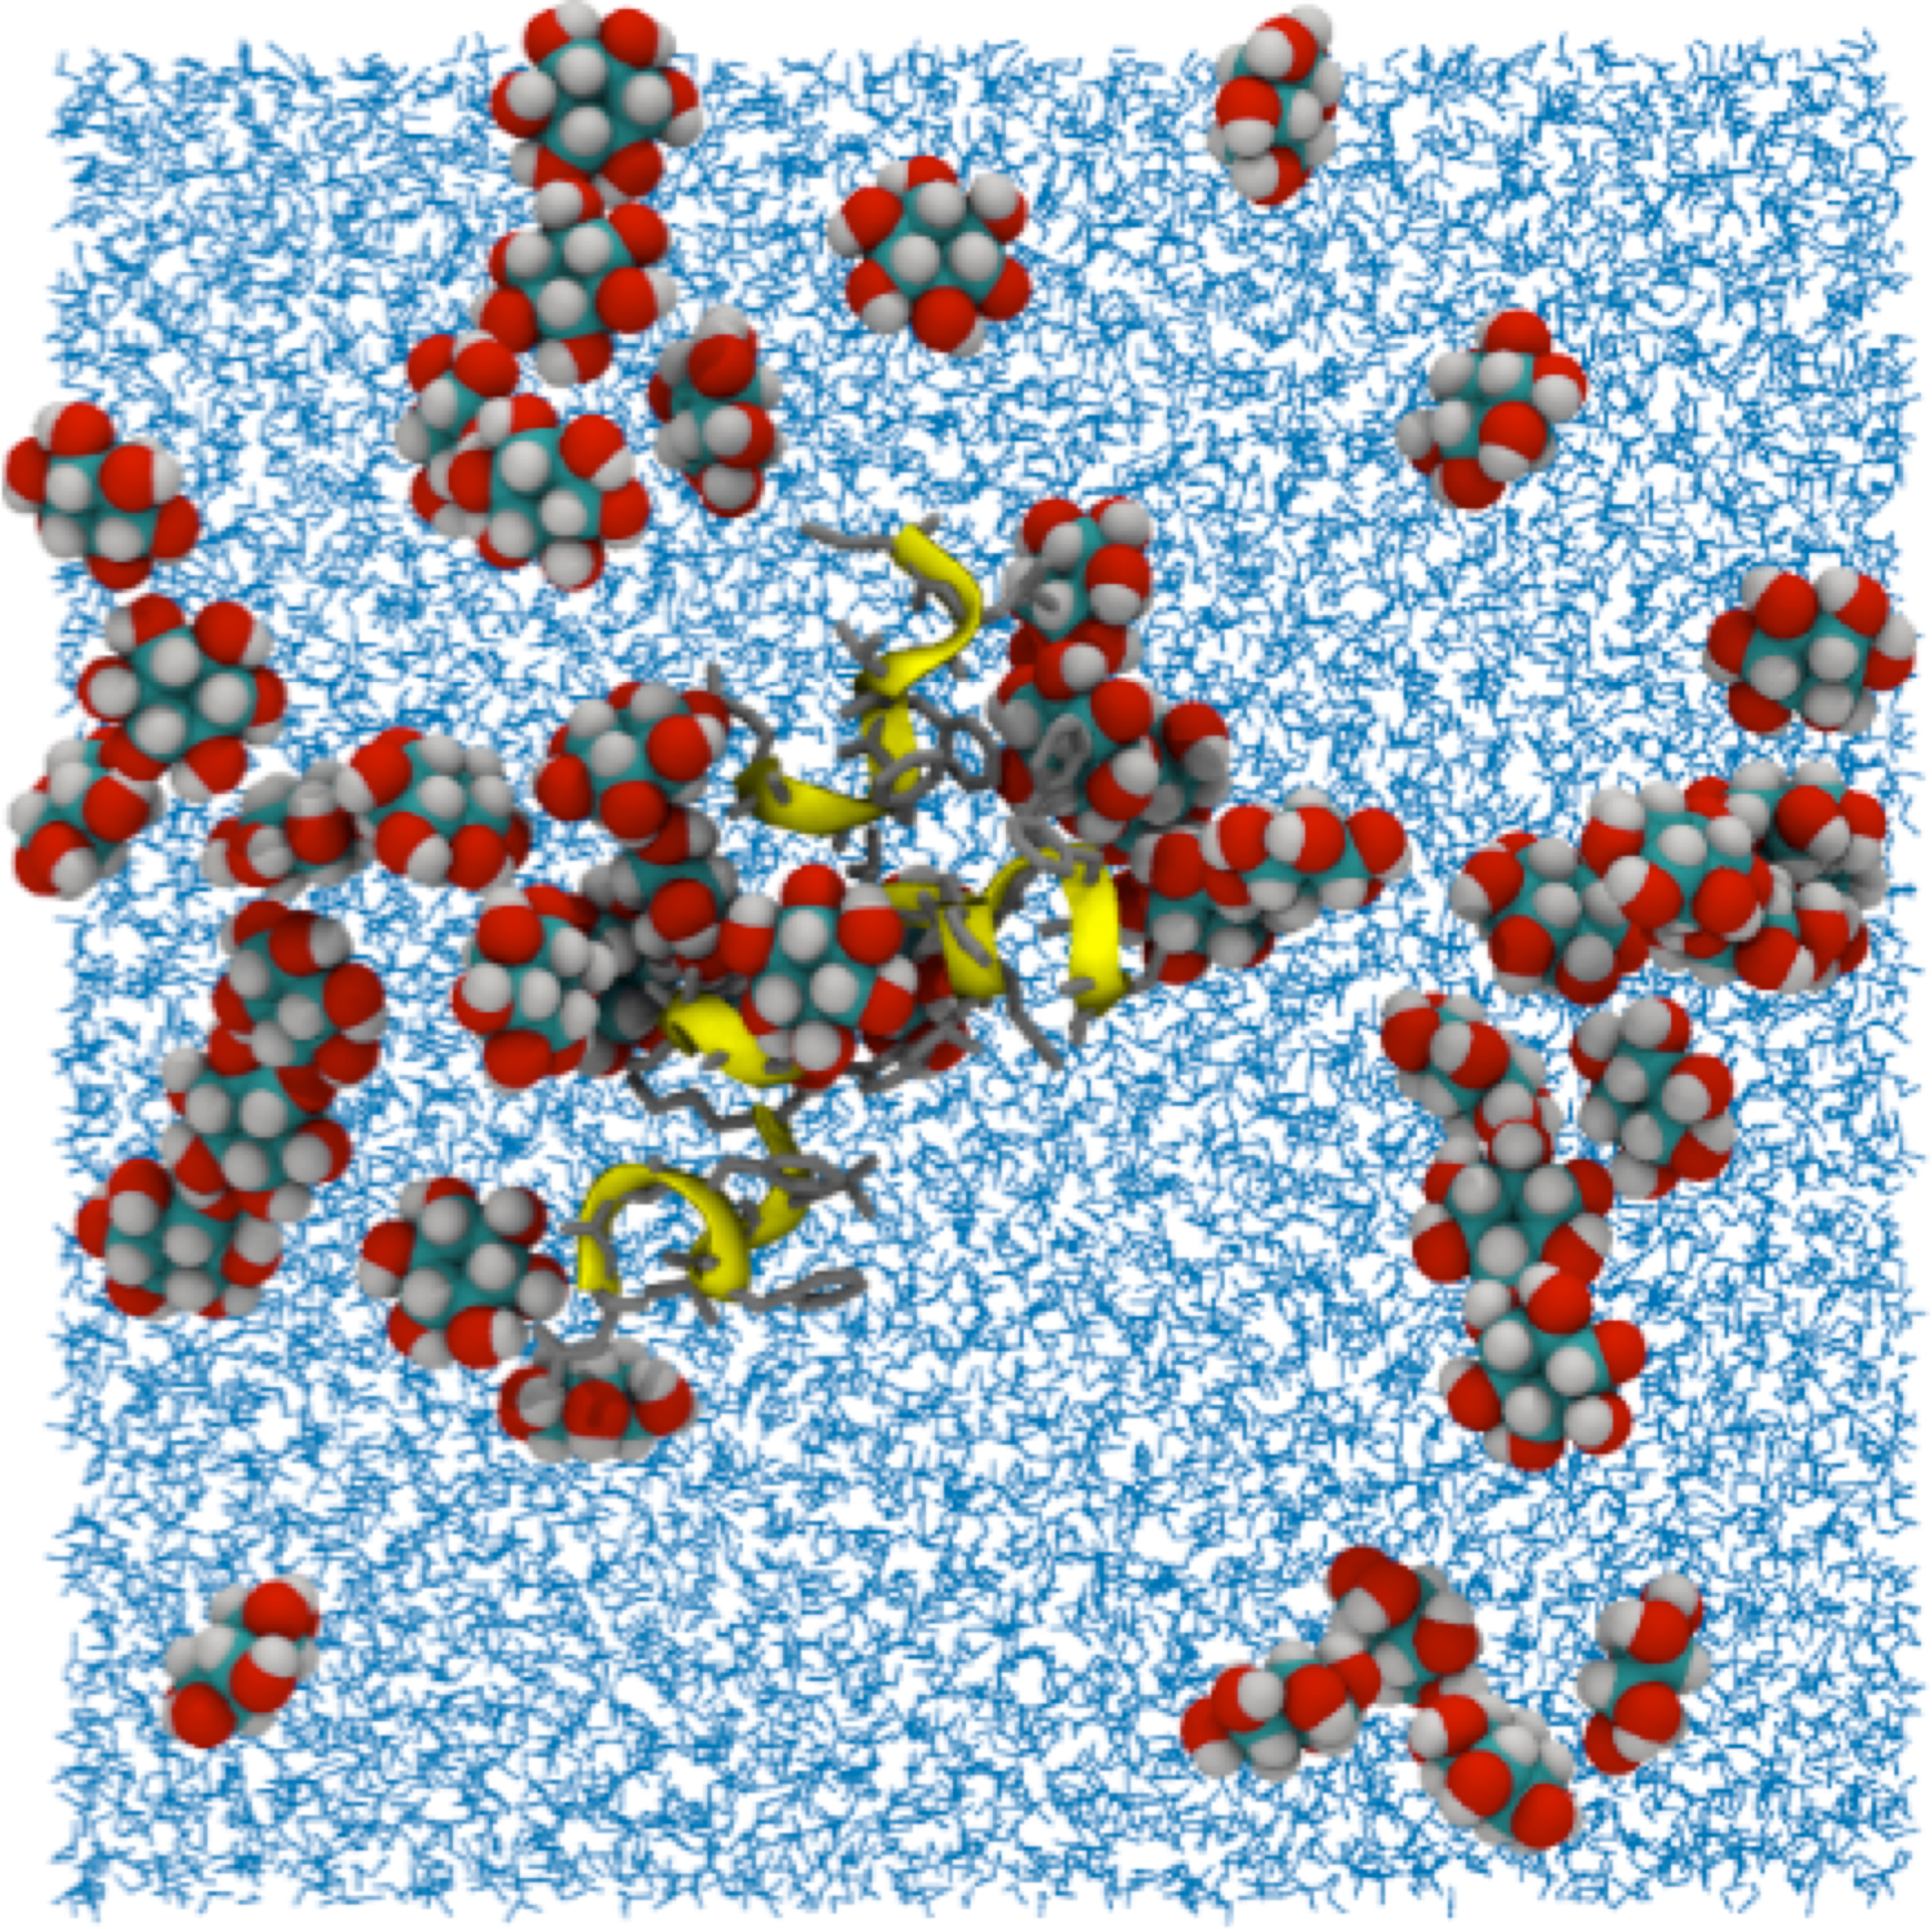
\includegraphics[width=5in]{figures/methods/simulation_box.pdf}
 \caption[An example of a MD simulation system]{An example of a MD simulation system.}
 \label{fig:simulation_box}
\end{figure}

Prior to performing production dynamics, which is what most of the results from a simulation will be based on, a short simulation to equilibrate the system is performed.  Equilibration is performed to allow the pressure and temperature of the system to stabilize. Here the stability of the protein is also validated to ensure that the protein structure has not grossly deviated (or unfolded) from the starting model.  

\begin{figure}
 \centering
 \includegraphics[width=5in]{figures/methods/equilibration.pdf}
 \caption[RMSD from the initial crystal structure calculated from an equilibriation]{Equilibration of the simulation system.}
 \label{fig:simulation_equilibration}
\end{figure}

\addcontentsline{toc}{section}{Bibliography}
\bibliographystyle{plain}
\bibliography{introduction}

%\section{Application of MD in structure-based drug discovery}
%
%% \1 (Why computational?) Can help us get protein dynamics is important for understanding protein function. We want to understand protein function because we want to be able to design drugs to cure diseases.
%
%% \1 A important application of MD simulation in biochemistry is the predicting of protein-ligand binding free energies.
%
%One application of MD simulations is in rational drug design. In recent years structure-based computer modeling of protein-ligand interactions have become a core component of modern drug discovery.  In early stage drug discovery, a target is identified along with putative binding sites.  Then, the structure of the target is determined using structural determination techniques such as NMR or X-ray crystallography.
%% [See Tom's thesis]
%Ligands which may act as potential drugs are expected to bind with a high affinity (low $K_d$) to the binding site. The goal is to discover,  high specificity inhibitors of a protein (usually an enzyme). In this process, the binding free energy of the ligand to its target is used to quantitatively evaluate how well a ligand binds. A crude estimate of the binding affinity can be obtained using computational docking methods, where the energetics of binding is typically estimated without accounting for either ligand or protein flexibility.  Although docking is fast, it is often inaccurate for identifying true drug candidates.
%
%With computer hardware becoming faster and cheaper, MD simulations can be used to rapidly prototype experimental ideas -- for example, one can perform computational alchemy, that is, ``mutate'' residues to test various hypotheses. Furthermore, simulations may be used to determine whether a chemical change will produce a more potent drug candidate. Currently, state of the art computational binding studies use MD simulations, where the protein and drug is allowed to relax and freely move about in the system. However, in the case of understanding a specific binding reaction often needed when developing an enzyme inhibitor, the ability to observe the relevant binding events is a low probability event on the timescale achievable by simulations. Therefore, a few enhanced techniques have been developed to accelerate this process.  They are briefly introduced below.
%
%\section{Free energy calculations}
%There are two advanced methods that have been developed for determining the absolute binding free energies in combination with MD simulations.
%
%% \3 Linear interaction energy -- Out of scope
%% \3 MM/PBSA - no explicit account for solvents -- Out of scope
%\subsection{Thermodynamic perturbation}
%This is the paper that I am taking most of the topics here\cite{Gilson:2007hz}
%
%\subsection{Thermodynamic integration}
%I actually have no idea what this is, and would be hard pressed to explain this properly.
%In this case, I don't think I should be covering these topics in my thesis.
%
%\subsection{Free energy perturbation}
%Alchemically change one molecule into another
%
%\section{Review of MD studies of amyloid inhibition by small molecules}
%% MD studies using brute-force sampling. Aid in medicinal chemistry by making suggestions for how to design new AD drugs.
%
%\begin{outline}
%	%  Excerpt from Transfer proposal
%	\1 In recent years, molecular dynamics simulations have been intensively used to investigate the molecular basis of the structure and stability of amyloid fibrils. 
%	
%	\1 MD simulations of Congo red binding have been done with the protofibril-like crystal structure composed of the segment GNNQQNY.\{Wu, 2007 \#621\}
%	
%	\1 A recent simulation study of an N-methylated peptide with A$\beta$16-22 models of amyloid aggregates has provided insight into the possible mechanism of action of peptide inhibitors of amyloid formation.\{Soto, 2007 \#597\} This peptide inhibitor was shown to preferentially bind monomers to form dimers, possibly acting to inhibit fibril formation by sequestering monomers. However, peptide-based inhibitors have poor pharmacological profiles as they are actively broken down by proteases in the stomach and are difficult to transport across the blood-brain barrier. In addition, these peptide inhibitors specifically target A$\beta$ and thus do not have the potential to treat multiple amyloid diseases.
%\end{outline}


% Scrap
% Motivate the use of MD simulations
% Describe the details of molecular dynamics simulations
% Review the basic derivations of MD simulation equations and why they work

% Molecular dynamics simulations are a useful tool to study the structure, dynamics, and interaction of biomolecules. 

% MD is a numerical algorithm which solves a system of Newtonian equations of motion, and provides as output the time-trajectory of atoms with femtosecond time resolution.

% To review before my defense

% Details of the mathematics (need to review the basic theory + Taylor series expansion) - get a book - tomorrow maybe?

% Why is MD correct? Describe the fundamental assumptions of MD. Here, I want to give the readers who aren't familiar with the methodological details of MD a sense of the rigorousness of MD.

% The assumption at a hand-wave level adapted from Tom's thesis

% - Relationship between force and energy 
% - Relationship between momentum and velocity 
% - Why numerical approach must be used (no analytical solution for N > 2)
% - How is the force field plugged into the general algorithm.






% \subsection{Setting up a MD simulation: practical aspects} - Here are some details to run a MD simulation of a biomolecular system.  Should I omit this from my introduction? This is not really essential in understanding the rest of my thesis, or is it? Perhaps this should go into an appendix instead -- this isn't interesting. The following steps are often used to setup and start a MD simulation system of a protein. First, a pre-determined structure, typically a coordinate structure from X-ray crystallography or NMR, or homology-modelling data. Then a force field and solvent is chosen.


%\section{Limitations of MD simulations}
% Rauscher:2010p5682,Rauscher:2009wr}  % Ref: DE Shaw and CN
% Schlick T (2010) Molecular modeling and simulation: an inter- disciplinary guide, interdisciplinary applied mathematics, vol 21, 2nd edn. Springer, New York


% Given the approximations of MD, MD is well-suited for probing the dynamics of complex systems on the timescale of picoseconds to seconds. ???

%Roughly speaking, one would like to run a simulation at least 10 times longer than the slowest important timescale in a system. Unfortunately, many biomolecular timescales exceed 1 ms, and in some cases by orders of magnitude (44).\cite{Zuckerman:2011dz} For molecular simulations to reliably predict, guide, and help explain experiment, these simulations require force fields of sufficient accuracy, adequate sampling of the relevant biomolecular motions (convergence) and a correct representation of the experimental conditions. Failures in any of these areas yield results which disagree with experiment.Until sampling is adequate, equilibrium properties computed from a simulation remain biased by the system�s starting state and no meaningful comparison with experiment is possible [6]. 

%% copied from Zukerman\cite{Zuckerman:2011dz}
%\textbf{Although routine explicit-solvent MD simula- tions are now four or five orders of magnitude longer (i.e., 100-103 ns currently), modern MD studies still appear to fall significantly short of what is needed for statistically valid equi- librium simulation (36, 38). Roughly speak- ing, one would like to run a simulation at least 10 times longer than the slowest impor- tant timescale in a system. Unfortunately, many biomolecular timescales exceed 1 ms, and in some cases by orders of magnitude (44).}
%% Other references that are relevant for sampling \cite{Grossfield:2009bn}
%
%% Copied from \cite{Mobley:2011ks}
%\textbf{For molecular simulations to reliably predict, guide, and help explain experiment, these simulations require force fields of sufficient accuracy, adequate sampling of the rel- evant biomolecular motions (convergence) and a correct representation of the experimental conditions. Failures in any of these areas yield results which disagree with experiment. 
%
%We may be tempted to blame disagreement with experiment on just one of these areas�force fields are perhaps the most common scapegoat, sometimes with good reason [1�5]�but any or all of the three may be a weak point. And, in some sense, adequate sampling is the weakest link. 
%
%Until sampling is adequate, equilibrium properties computed from a simulation remain biased by the system�s starting state and no meaningful comparison with experiment is possible [6]. 
%
%With an inadequate force field or a poor representation of the experimental conditions, results will disagree with experiment, but will be robust and improvement is relatively easy, but not so with inadequate sampling.}
%
%% copied from Sarah's thesis
%\textbf{Achieving complete (or even adequate) conformational sampling is one of the key challenges in biomolecular simulations.\cite{Gnanakaran:2003vh} The energy landscape of most biomolecules is �rugged� and the source of this ruggedness is two-fold. The energetic barriers separating accessible states are often larger than the available thermal energy, and there are typically a large number of states to be sampled. The timescales of many biomolecular processes, such as protein folding, are still far beyond the reach of our current computational capability, which is generally limited to the 10-8-10-7 s timescale for continuous simulations. For example, even the folding of small domains or secondary structure elements, such as ?-hairpins and mini-proteins, occur on the 1-10 ?s timescale.1 
%
%Consequently, conventional or �brute force� molecular dynamics (MD) alone is often insufficient to achieve complete Boltzmann sampling of the important states of many biologically relevant systems. For this reason, generalized-ensemble algorithms have become popular tools for conformational sampling.}

% Topics that I'm not going to discuss
%Evaluating the convergence of simulations is still a challenge - I don't want to  go into this as this is out of the scope of my thesis.
%Limitations in the accuracy of current force fields - Don't talk about this .. but this will probably come up during the defense regardless.
\chapter{Results}

In this chapter, the hydration of proton uptake pathways and the structural fluctuations (or conformational isomerization) of the D-channel in wildtype and mutant cytochrome \emph{c} oxidase embedded in a lipid bilayer are analyzed.

\section{Stability and relaxation of the simulation system}
\label{sec:results-relaxation}

The root-mean-square deviation (RMSD) of backbone heavy atoms from the initial conformation of the four unbiased simulation systems (Fig. \ref{fig:equilibration_relaxation}) shows that these systems are stable after approximately 20 ns of simulation. The RMSD remains within 2 Å from the starting structures, as a result of thermal fluctuations. In comparison, the RMSD of backbone atoms in the finite-sized simulation system used previously was within 0.3 Å due to the harmonic restraints imposed on the atoms.

In the next sections of this chapter, we revisit the equilibrium properties of the D-channel in the absence of spatial restraints made possible by the presence of explicit solvent, with periodic boundary conditions mimicking an infinite system.
%Figure \ref{fig:equilibration_relaxation}B shows the contrast between D-channel backbone (residues N139, N121, N207, S142, S200, S201, S197, and E286) relaxation in the biased system used in the current study, and unbiased system used previously. This is included to illustrate how the biased system constrains the backbone of the D-channel residues, compared to the unbiased system which is allowed to equilibrate freely.

\begin{figure}[htbp]
\centering
\includegraphics{figures/equilibration_relaxation/backbone.png}
\caption[Deviation from initial structure in molecular dynamics simulations of cytochrome \emph{c} oxidase.]{Equilibration plots showing backbone (C, C$_\alpha$, N) RMSD of four variants of the unbiased C\emph{c}O system embedded in a solvated DPPC bilayer.}
\label{fig:equilibration_relaxation}
\end{figure}

\section{Conformational isomerization of residue 139}
\label{sec:results-isomerization}

In this study, The potential of mean force (PMF) for the rotation around the residue's $\chi_1$ dihedral angle is calculated in four variants of C\emph{c}O: wildtype (N139), N139D, D132N, and N139D/D132N. As found in earlier work \cite{Henry:2009p4543,Henry:2011p10221}, residue 139 exhibits three metastable rotameric states: ``outfacing'', ``closed'', and ``open''. In the ``closed'' state, the side chain of residue 139 prevents the formation of a hydrogen-bonded water wire \cite{Henry:2009p4543}. In the ``open'' state, the side chain moves out of the way, allowing a water wire to form. In the ``outfacing'' state, the residue's side chain points towards the entrance of the D-channel, with the terminal amide or carboxylate group located in the ``vestibule'' region of the D-channel. Representative snapshots of the D-channel for the three known metastable states are shown in Fig. \ref{fig:dchannel_snapshots}.

\begin{figure}[htbp]
\centering
\includegraphics{figures/chi1_pmfs_unbiased/chi1_unbiased_pmfs.png}
\caption[PMF for the $\chi_1$ rotation of the side chain of residue 139 in wildtype and mutant cytochrome \emph{c} oxidase.]{PMF for the $\chi_1$ rotation of N139 (blue), N139D (red), N139D the D132N/N139D double mutant (green) and N139 in the D132N mutant (cyan). All PMFs are aligned to the wildtype closed state ($\Delta G = 0$ kcal/mol). The three metastable states are labeled above the graph.}
\label{fig:pmf_chi1_unbiased}
\end{figure}

\begin{figure}[htbp]
\centering
\includegraphics{figures/139_rotamers/dchannel_snapshots.png}
\caption[Representative snapshots of the D-channel for three metastable conformations of residue 139.]{Representative snapshots of the D-channel for three metastable conformations of residue 139: (a) ``closed'' (crystallographic) conformation of N139 in the wildtype enzyme; (b) ``open'' conformation of the N139D single mutant; and (c) ``outfacing'' conformation of N139D in the D132N/N139D double mutant. Water molecules present in or near the D-channel are shown in spherical representation together with licorice representations of the side chains of residues 132, 139 and 286. The C$_\alpha$ trace of the protein is depicted as ribbons.}
\label{fig:dchannel_snapshots}
\end{figure}

In the wildtype protein, the ``closed'' state, in which the side chain of residue 139 blocks the water wire, is the most energetically favourable. The ``outfacing'' and ``open'' states of the wildtype protein are equally energetically favourable (within 1 kcal/mol). The PMF of the D132N single mutant nearly overlaps with that of wildtype, though its ``open'' state is 2.5 kcal/mol more favourable than its ``outfacing'' state. The single N139D and double N139D/D132N mutants are almost indistinguishable. They are similarly favourable (within 2 kcal/mol) in their ``closed'' and ``open'' states, but overall they both favour the ``outfacing'' state by 4 kcal/mol.

\begin{figure}[htbp]
\centering
\includegraphics{figures/chi1_pmfs_comparison/pmf_comparison.png}
\caption{Comparison of PMFs for $\chi_1$ rotation of residue 139 between the biased (finite-size) and new unbiased simulation systems.}
\label{fig:pmf_chi1_comparison}
\end{figure}

There are a few notable differences between the results from the biased and unbiased simulation systems (Fig. \ref{fig:pmf_chi1_comparison}). Upon removal of conformational restraints, the ``outfacing'' state becomes more favourable for all variants in the unbiased system. Most notably, in the N139D mutant the free energy of the ``outfacing'' state decreases by 9 kcal/mol relative to that of the closed state and becomes the most probable conformer. In the biased system, electrostatic repulsion between residues D132 and D139 (in the N139D single mutant) may have affected the stability of the ``outfacing'' conformer. However, in the unbiased system, thermal fluctuations resulted in relaxation of the D-channel, resulting in an increase in the distance between the C$_{\gamma}$ atoms of residue 132 and 139 to 9.8 Å, compared to 8.6 Å in the wildtype system, and 7.55 Å in the crystallographic structure (Table \ref{tbl:gamma_distances}) and thereby reducing the pairwise coulombic repulsion by 5 to 10 kcal/mol in the single mutant N139D.

\begin{table}
    \begin{center}
    \begin{singlespaced}
    \caption{Average distance between C$_{\gamma}$ of residues 132 and 139 in the outfacing state of residue 139.}
    \vspace{10pt}
    \label{tbl:gamma_distances}
    \begin{tabular}{lc}
    System  & C$_{\gamma}$ Distance \\
    \hline
    Wildtype & 8.6 $\pm$ 0.6 \\
    D132N & 9.3 $\pm$ 0.3 \\
    N139D & 9.8 $\pm$ 0.6 \\
    N139D/D132N & 9.0 $\pm$ 0.7 \\
    \hline
    \end{tabular}
    \end{singlespaced}
    \end{center}
\end{table}

\section{Hydration analysis of equilibrium trajectories}
\label{sec:results-hydration}

\begin{figure}[htbp]
\centering
\includegraphics{figures/hydration/hydration.png}
\caption[Analysis of hydration of the D-channel and K-channel.]{Analysis of hydration of the D-channel (left) and K-channel (right). The solid lines in each graph show the normalized distributions of water molecules along the lengths of the D- and K-channel cylinders. The dotted lines show the mean cumulative sums of water molecules starting from the entrance of each channel. A representative snapshot of water in each channel is displayed above each graph. In A and B, residues N/D132, N/D139, and E286 are shown from left to right. In C, residues G312, K362, and Fe$_{a3}$ are shown from left to right. Snapshot A depicts N139 in its ``closed'' conformation, B shows the double mutant (N139D/D132N) with ``outfacing'' residue D139, and C shows the wildtype hydrated K-channel.}
\label{fig:hydration}
\end{figure}

Normalized water distributions and cumulative sums in the D- and K-channels were calculated from the equilibration trajectories of each variant (Fig. \ref{fig:hydration}). Water distributions of the D-channel in the N139 variants (wildtype and D132N, Fig. \ref{fig:hydration}A) show that 10-12 water molecules occupy the channel on average. The distributions in the same figure clearly show the bottleneck occupied by residue N139 as described by Henry et al. (2009) \cite{Henry:2009p4543}. On the other hand, the N139D variants (Fig. \ref{fig:hydration}B) show no gap in D-channel hydration, suggesting that the side chain of residue 139 does not prevent the formation of a nearly continuous water wire. As a result, 2-4 more water molecules enter the D-channel as shown by the cumulative sum plots. These data, being from unbiased simulations, represent D-channel hydration with residue 139 in its most favourable orientation (see section \ref{sec:results-isomerization} below for details): ``closed'' for N139, and ``outfacing'' for D139. In addition, the dependence of hydration on the orientation of residue 139 was also analyzed (Figs. \ref{fig:hydration_n139_allchi1} and \ref{fig:hydration_n139d_allchi1}). These results show a small but non-zero probability of hydration in the bottleneck in wildtype when residue N139 is ``outfacing'' or ``open'', also consistent with earlier work \cite{Henry:2009p4543}. No significant correlation is observed between the orientation of residue N139D and hydration of the D-channel in the N139D single mutant.

Equilibrium hydration of the K-channel was observed in all simulation systems. The results show a consistent distribution across the four systems, except between 15 and 25 Å away from the entrance of the channel. The distribution supports the notion that the K-channel contains a stable water wire, consistent with previous work predicting the K-channel to be a functional proton channel \cite{Tomson:2003p10255,Ganesan:2010p8417}.

% hydration of WT in outfacing, closed and open states
\begin{figure}[htbp]
\centering
\includegraphics{figures/hydration/hydration_analysis/chi1_wt/all_chi1_wt.png}
\caption[Hydration analysis of the D-channel in the wildtype (N139) when the side chain is in each of the three metastable states: outfacing, closed, and open.]{Hydration analysis of the D-channel in the wildtype (N139) when the side chain is in each of the three metastable states: outfacing, closed, and open. The solid lines show the normalized distributions of water molecules along the lengths of the D-channel cylinders. The dotted lines show the mean cumulative sums of water molecules starting from the entrance of each channel.}
\label{fig:hydration_n139_allchi1}
\end{figure}

% hydration of N139D in outfacing, closed and open states
\begin{figure}[htbp]
\centering
\includegraphics{figures/hydration/hydration_analysis/chi1_n139d/n139d_all_chi1.png}
\caption[Hydration analysis of the D-channel in the N139D single mutant when the side chain is in each of the three metastable states: outfacing, closed, and open.]{Hydration analysis of the D-channel in the N139D single mutant when the side chain is in each of the three metastable states: outfacing, closed, and open. The solid lines show the normalized distributions of water molecules along the lengths of the D-channel cylinders. The dotted lines show the mean cumulative sums of water molecules starting from the entrance of each channel.}
\label{fig:hydration_n139d_allchi1}
\end{figure}

\section{Thermodynamics of \ce{K^+} translocation through the D-channel}
\label{sec:results-kplus}

\begin{figure}[htbp]
\centering
\includegraphics{figures/kbinding_pmfs/combined_pmf.png}
\caption[PMFs for \ce{K^+} from bulk water, through the D-channel ``vestibule'' to residue E286 in four variants.]{PMFs for \ce{K^+} from bulk water, through the D-channel ``vestibule'' to residue E286 in four variants. Each variant's PMF is the average of 5 independent replica sets. The error is standard deviation between the individual PMFs. A \ce{K^+} ion, and residues D132, N139, and E286 (wildtype) are shown at the top as a reference. The four regions (A-D) along the reaction coordinate are also shown for reference. All PMFs are aligned on the bulk water region, where $\Delta G = 0$ kcal/mol.}
\label{fig:pmfs_kbinding}
\end{figure}

It has been proposed that the highly-conserved residue N139 acts as a barrier to cations, imparting proton selectivity to the D-channel \cite{Henry:2009p4543}. During a simulation of the N139D protein, a \ce{K^+} ion was observed within the ``vestibule'' region of the D-channel. This finding was completely unexpected and led us to investigate \ce{K^+} binding to the D-channel of C\emph{c}O variants.

The PMFs of four systems for \ce{K^+} translocation from bulk water through the D-channel to residue E286 are shown in Fig. \ref{fig:pmfs_kbinding}. Each PMF shown is the average of five PMFs, one per replica set, for each individual system. Error bars represent the standard deviation between the PMFs in each set. For convenience, four regions along the reaction coordinate are defined: A (-50 to -32 Å), B (-32 to -24 Å), C (-24 to -16 Å), and D (-16 to 0 Å). Snapshots of the D-channel (in wildtype and the N139D single mutant) with the cation in each of the four regions is shown in Fig. \ref{fig:kbinding_snapshots}.

% SNAPSHOTS of each region -27, -21, -13, -5
% -27: 63, 95, 114
% -21: 49, 58
% -13: 51, 56, 76, 107
% -5: 1, 27, 31
\begin{figure}[htbp]
\centering
\includegraphics{figures/kbinding_snapshots/snapshots.png}
\caption[Snapshots of each of the four regions of the reaction coordinate in wildtype and N139D D-channels showing residues D132, N139 (or D139), and E286.]{Snapshots of each of the four regions of the reaction coordinate in wildtype and N139D D-channels showing residue D132, N139 (or D139), and E286. The \ce{K^+} cation is shown as the purple sphere.}
\label{fig:kbinding_snapshots}
\end{figure}

Region A contains bulk water, in which the PMF is flat, as \ce{K^+} diffuses freely through water. In region B (the ``vestibule'' region) the cation approaches the ``proton antenna'', which contains residue 132. There is a clear difference in free energy between the variants containing D132 (wildtype and N139D) and D132N (D132N, and N139D/D132N), suggesting that \ce{K^+} is repelled when D132 is replaced by N, but attracted to the mouth of the D-channel in the N139D single mutant. In the double mutant, $\Delta G$ is approximately zero, suggesting that the entrance to the D-channel is neither attractive nor repulsive to \ce{K^+}. In region C (which contains the top of the ``vestibule'' region), the PMFs of the N139 and D139 variants begin to diverge dramatically. The N139 bottleneck creates a 25 kcal/mol barrier in both wildtype and D132N variants. In the double mutant (N139D/D132N) we see a barrier of 5 kcal/mol, which drops to 1 kcal/mol as the cation approaches residue D139. In contrast, the single N139D mutant shows a monotonic decrease in free energy for the movement of \ce{K^+} through this region. Past residue 139, in region D, the cation is hydrated within the ``fluid-like'' region of the D-channel, and is attracted by the deprotonated glutamic acid, E286, in all the variants considered.

\begin{figure}[htbp]
\centering
\includegraphics{figures/kbinding_chi1z/chi1z.png}
\caption[Density maps showing the distribution of residue 139's $\chi_1$ dihedral angle as the \ce{K^+} ion translocates through the D-channel.]{Density maps showing the distribution of residue 139's $\chi_1$ dihedral angle as the \ce{K^+} ion translocates through the D-channel. Data from the two N139 variants (wildtype and D132N) are shown on the left and data from the two N139D systems are shown on the right. The three metastable states of $\chi_1$ are labeled above each heatmap. The shaded bar across the figures indicate the location of the c$_\alpha$ of residue 139, relative to the C$_\alpha$ atom of E286 (at position 0).}
\label{fig:kbinding_chi1z}
\end{figure}

It is clear from the PMFs that residue N139 blocks \ce{K^+} when it is in the ``closed'' state. To better understand how the cation's position affects the orientation of residue 139, the distribution of residue 139's $\chi_1$ dihedral angle was plotted versus the position of the cation along its reaction coordinate (Fig. \ref{fig:kbinding_chi1z}). These data show that the cation has an influence over residue 139's $\chi_1$ dihedral angle when it is in closer proximity to the side chain (region B of Fig. \ref{fig:pmfs_kbinding}). In the N139 systems, the residue flips into its ``open'' orientation, and then back into its ``closed'' orientation as the cation approaches the N139 side chain. In the N139D systems, the side chain is further stabilized in its ``outfacing'' orientation when the cation is in the ``vestibule''. The side chain follows the cation along its path once they are closer in proximity, leading to a stable ``closed'' state as the cation enters the ``fluid-like'' region of the channel.

These results suggest that residue N139 acts as a barrier for cations such as \ce{K^+}, a function which is abolished in the N139D single mutant. The double mutant seems to show a 5 kcal/mol barrier in the ``vestibule'' region, but whether this can prevent \ce{K^+} from entering the channel may depend on the concentration of \ce{K^+}. As discussed in the next chapter, we propose that this barrier may play a role in the D-channel's proton selectivity mechanism.

\subsection{Dissociation constant for \ce{K^+} binding to the D-channel ``vestibule''}
\label{sec:results_dissociation_constants}

The dissociation constant for \ce{K^+} binding to the D-channel ``vestibule'' was calculated in four systems from the PMFs above (Fig. \ref{fig:pmfs_kbinding}) as per the methods in section \ref{sec:dissociation_constants}. The binding site (``vestibule'') region of the PMF is defined to be between -32 Å and -20 Å ($z_{min}$ and $z_{max}$, respectively). The results are listed in Table \ref{tbl:dissociation_constants}.

\begin{table}
    \begin{center}
    \begin{singlespaced}
    \caption{$K_d$ for \ce{K^+} binding to the D-channel ``vestibule'' in four C\emph{c}O variants.}
    \vspace{10pt}
    \label{tbl:dissociation_constants}
    \begin{tabular}{lc}
    Variant & $K_d$ of \ce{K^+} \\
    \hline
    Wildtype & 41.82 M \\
    N139D & 0.11 mM \\
    D132N & 24989.51 M \\
    N139D/D132N & 75.07 M \\
    \hline
    \end{tabular}
    \end{singlespaced}
    \end{center}
\end{table}

% dG = -RTlnK K = e^{-dG/RT}
% R = 0.00198722 kcal/mol*K
% T = 323.15 K

% [K+ unbound] = 3.3 M
% from the restrained cylinder (1 atom in 502.66 Å^3)
% P_unbound = 1/502.66 Å^3

% [S]   = (1/6.022*10^23) / (V Å3)*(1*10^-27 L)
%       = 1660.577881 * 1/V

% at 1/2 occupancy, P_bound/P_unbound = 1, so K = [S] at 1/2 occupancy
% C_unbound = 1 molecule / V_unbound = 1 / (length * pi * 4^2)
% C_unbound = 1 molecule / (P_bound * pi * R^2)
% P_unbound = 1 / V_unbound

% at 1/2 occupancy
% P_bound = P_unbound 
% P_unbound = 1 / (L*16pi)
% P_bound = 1 / (L_EC *16pi)
% L_EC = 1/(P_bound*16pi)

% V_EC = L_EC*16pi = 1/P_bound

% P_bound
% Wildtype          0.79        V = 39.71           [S] = 41.82 M
% N139D             314368.82   V = 15801900.41     [S] = 0.11 mM
% D132N             0.001322    V = 0.066451        [S] = 24989.51 M
% N139D/D132N       0.44        V = 22.12           [S] = 75.07 M


\chapter{Discussion}

% summary
%   new simulation system of CcO based on...
%   hydration
%   isomerization of residue 139
%   loss of a cation barrier
%   new hypothesis for decoupling and recoupling?
Previous computational studies from our laboratory have led us to propose that residue N139, a highly conserved residue within the D-channel, plays a role in proton gating and selectivity \cite{Henry:2009p4543,Henry:2011p10221}. Single-point mutations of N139, such as N139D and N139A, have been shown to inhibit proton pumping while modulating rate of redox activity \cite{Pawate:2002p5614,Namslauer:2003p6853}. Residue D132, another conserved residue at the entrance of the D-channel, has been proposed to act as a ``proton antenna'' that recruits protons from bulk water into the D-channel \cite{Mills:2000p4585,Henry:2009p4543}. Single-point mutations of D132, such as D132N and D132A, also decouple the protein, presumably by decreasing proton affinity of the D-channel \cite{Fetter:1996p5464,Henry:2011p10221}. Interestingly, the combination of the two mutants results in a functional double mutant (N139D/D132N) \cite{Branden:2006p9874}. This decoupling/re-coupling phenomenon may help us understand the molecular basis of proton pumping, which is why we are studying these mutants. Some mutations have been shown to affect the p$K_a$ of residue E286, the ``proton shuttling'' residue at the top of the D-channel, which is responsible for passing on chemical protons to the binuclear centre (BNC) and vectorial protons to the proton-loading site (PLS) \cite{Namslauer:2003p6853,Han:2006p5624,Branden:2006p9874,Fadda:2008p5482,Pisliakov:2008p7746,Lee:2010p8614}. Certain mutations have also been found to affect equilibrium hydration within the channel \cite{Tashiro:2005p7174,Sugitani:2009p5715,Henry:2009p4543}. A recent study based on computer simulations suggested that the double mutant restores wildtype electrostatic properties in the D-channel via a specific adjustment in the orientation of residue N139D, thus reenabling proton pumping \cite{Henry:2011p10221}. While this study shows how conformational fluctuations and electrostatics play a key role in the decoupling mechanism, it does not fully explain the modulation of redox activity in these mutants.

In this thesis, computer simulations are used to further investigate gating and selectivity in the D-channel of wildtype and mutant oxidase. To expand on previous work done in our laboratory over the past 3 years \cite{Henry:2009p4543,Henry:2011p10221}, a new unbiased model of C\emph{c}O from \emph{R. sphaeroides} \cite{SvenssonEk:2002p5595} embedded in a hydrated lipid bilayer was constructed and used to study equilibrium hydration, conformational dynamics, and cation binding to the D-channel. The new simulation system is two orders of magnitude larger than the one used previously (250,000 atoms vs 900 atoms) and it would have been nearly impossible to study at length without large computational resources such as SciNet, as over 5 million CPU-hours were required. The challenges of using computer simulations to study the equilibrium properties of proteins stem from the fact that conformational changes occur over a wide range of timescales, a problem which is compounded by the slow relaxation of the lipid bilayer \cite{Neale:2011p2011712}. As a result, free energy calculations in membrane proteins present a challenge, as the convergence of such calculations is related to the inherent relaxation timescales of the system. As such, the accuracy of combined molecular dynamics/free energy calculations depends on the properties of the system under consideration. If a given simulation is much longer than the slowest relevant exchanges or relaxation times, brute-force sampling is adequate. However, if the slowest events occur on timescales longer than that of the simulation, enhanced sampling techniques such as umbrella sampling (US) must be used to study the system's distinct substates. The size of the unbiased system studied in this thesis precludes the use of brute force sampling for studying conformational dynamics of individual residues as well as cation translocation through the D-channel (sections \ref{sec:results-isomerization} and \ref{sec:results-kplus}). On the other hand, water rapidly equilibrated in the uptake proton pathways known as the D- and K-channels, so that hydration (section \ref{sec:results-hydration}) was analyzed from the unbiased trajectories of each system, resulting in equilibrium distributions of water in the D- and K-channels.

\section{Conformational isomerization of residue 139}

The analysis of conformational isomerization of the side chain of residue 139 in the unbiased simulation system resulted in a few notable differences compared to previous work done using the biased system. The ``outfacing'' state was shown to be significantly more favourable across all systems. Interestingly, the single N139D mutant was shown to be as favourable as in the double mutant (N139D/D132N) in its ``outfacing'' state, in which it is the prevalent conformer. In earlier work it was suggested that electrostatic repulsion between the carboxylate groups of residues 132 and 139 destabilized the ``outfacing'' state in the N139 single mutant \cite{Henry:2011p10221}. In the unbiased system there was an increase in the average distance between residues D132 and N139D of up to 3 Å, likely as a result of electrostatic repulsion between the two side chains. Importantly, the stabilization of the ``outfacing'' state in the N139D and N139D/D132N mutants still supports our previous model for decoupling and re-coupling \cite{Henry:2011p10221} as explained below.

\section{Hydration and gating of proton channels}

In Henry et al. (2009) \cite{Henry:2009p4543}, functional hydration of the D-channel was examined in detail and two regions of the D-channel were defined in terms of water mobility: the ``solid-like'' (0-8 Å) and ``fluid-like'' (10-35 Å) regions. The wildtype cumulative sum data from the new unbiased system (Fig. \ref{fig:hydration}A) shows that there are between two and three water molecules in the ``solid-like'' region, and between eight and nine water molecules in the ``fluid-like'' region, consistent with previous findings \cite{Henry:2009p4543}. Hydration of the D-channel in the N139A single mutant (Fig. \ref{fig:hydration_n139a}) is also consistent, as both studies indicate that there is no gap in the water wire.

Hydration of the K-channel was observed for the first time, supporting the hypothesis that the K-channel does indeed act as a functional proton channel \cite{Tomson:2003p10255,Ganesan:2010p8417}. These results only pertain to a single redox state of the protein (the R state). Changes in redox state may affect hydration, especially of the K-channel, as proton uptake from the N-side is only required for a few state transitions, and continuously hydrated channels may cause proton back-leak and pump malfunction. Given that we know very little about the K-channel, future work should examine hydration using a method similar to that in Henry et al. (2009) \cite{Henry:2009p4543}, whereby the changes in free energy between hydration states are determined in different catalytic states of the system.

The data on proton channel hydration presented here support some preexisting data, specifically concerning the existence of a dehydrated bottleneck at residue 139 which is thought to be functionally relevant as part of the N139 gating mechanism \cite{Henry:2009p4543}. Henry et al. (2009) found that, in residue 139's ``open'' state, the water wire gap can be occupied by a water molecule. In the ``closed'' state, the gap is occupied by the side chain of N139. This suggested that the residue may control the rate at which protons travel through the D-channel by repeatedly opening and closing the gap in the water wire \cite{Henry:2009p4543}. Data from the current study on conformational isomerization was used to determine whether the side chain orientations of residue N139 (and N139D) correlate to changes in equilibrium hydration of the D-channel. No significant correlation was observed in the N139D mutant (Fig. \ref{fig:hydration_n139d_allchi1}), suggesting that gating does not occur in the N139D single mutant. In the wildtype protein, there is a non-zero (but low) probability of hydration in the same region for the ``open'' and ``outfacing'' states (Fig. \ref{fig:hydration_n139_allchi1}). This particular finding corroborates with results from Henry et al. (2009) \cite{Henry:2009p4543}, such that the ``open'' state can be hydrated. The probability of finding a water molecule in the gap when the side chain is ``open'' may be significantly lower than expected, which would make such an event less likely to occur in the relatively short simulations of the unbiased model (ie dependent on equilibration times). In addition, hydration of the bottleneck may depend on the presence of a proton in the vestibule region. Further investigation may be required to determine the gating mechanism in the unbiased model.

\section{Implications for Proton selectivity of the D-channel}

Previous experimental work has suggested that \ce{Zn^{2+}} inhibits proton pumping in cytochrome \emph{c} oxidase by blocking proton uptake through D-channel \cite{Kannt:2001p8408,Aagaard:2002p8410,Kuznetsova:2005p8380,Faxen:2006p8398,Francia:2007p8388,Qin:2007p8387,Muramoto:2007p8383}. Based on an earlier simulation study of functional hydration in the D-channel, it was also postulated that the highly-conserved residue N139 acts as a barrier to cations, imparting proton selectivity to the D-channel \cite{Henry:2009p4543}. Proton selectivity in the D-channel is a requirement for the function of C\emph{c}O as the effective concentration of \ce{K^+} is many orders of magnitude higher than that of \ce{H^+} at physiological conditions. This work calls attention to this requirement which has been underappreciated up to this point in the literature on C\emph{c}O. 

During the equilibration run of the N139D single mutant in the presence of 0.15 M \ce{KCl}, a \ce{K^+} cation was observed to bind in the vestibule region of the D-channel. In addition, the hydration analysis of the D-channel in the N139D single mutant showed no evidence of a water wire gap (Fig. \ref{fig:hydration}). These findings led us to investigate the thermodynamics of \ce{K^+} translocation through the D-channel. PMFs describing the free energy for the translocation of \ce{K^+} from bulk water through the D-channel were calculated for multiple C\emph{c}O variants. In the results obtained for wildtype oxidase, the relative free energy difference between the vestibule region and bulk water is approximately 0 kcal/mol, suggesting that a \ce{K^+} cation can freely diffuse to the entrance of the D-channel. However, the energetic barrier observed in the vestibule (in wildtype and D132N proteins) is likely to prevent \ce{K^+} from entering further into the channel. These results support claim made by Henry et al. (2009), who suggested that the hydration bottleneck created by residue N139 may play a role in proton selectivity by excluding other monovalent cations from the D-channel \cite{Henry:2009p4543}. The most striking observation from the results obtained for the N139D single mutant is the lack of any cation barrier. This finding suggests that \ce{K^+} can spontaneously enter the D-channel and travel to residue E286. The driving force is likely to be the electrostatic interaction between the cation and the deprotonated side chains of residues D132, D139, and E286, in addition to the hydration state of the channel. In the charged, deprotonated state, E286 acts as a sink for cations, and I expect that when E286 is protonated, the cation will remain within the lower part of the D-channel (in the antenna or vestibule sites), based on earlier unpublished electrostatic calculations done by Yu, Chakrabarti, and Pomès. There is a desolvation penalty for \ce{K^+} to enter the channel, but hydration of the bottleneck alone may not be sufficient for \ce{K^+} to bind to the vestibule. For example, our results show that the N139A single mutant has a cation barrier despite being hydrated at the bottleneck (Figs. \ref{fig:hydration_n139a} and \ref{fig:pmfs_kbinding_n139a}). 

Overall, these findings suggest that the water/cation bottleneck created by residue N139 may play a significant role in proton selectivity in the D-channel. Further investigation on both the theoretical and experimental fronts is warranted.
% Chi1 & K+ distribution?

\section{Experimental relevance of \ce{K^+} and a potential artifact of experimental protocols: A testable hypothesis}

\ce{K^+} is a major intracellular cation in both bacterial and eukaryotic cells \cite{Epstein:2003p10379}. It plays a critical role in the maintenance of structural integrity of the cell by maintaining osmolarity. It is also thought to be responsible for maintaining the structural integrity of the mitochondria \cite{Garlid:2003p10324}. It turns out that the standard experimental protocols used to study proton pumping in C\emph{c}O involve buffers containing 40 to 100 mM \ce{K^+}, and the presence of \ce{K^+} is a critical part of the experimental design \cite{Hosler:1992p6662,Fetter:1995p6852,Namslauer:2003p6853,Lee:2009p8180,Namslauer:2010p9850,Zhu:2010p8237,Lee:2010p8614}. Valinomycin, a \ce{K^+} ionophore, is used to prevent the buildup of electrochemical membrane gradients in studies concerning the coupling of proton pumping to redox activity (Fig. \ref{fig:valinomycin_cccp}) \cite{Namslauer:2003p6853}. With valinomycin, the net proton release to the ``outside'' of the vesicles can be monitored. CCCP (carbonyl cyanide $m$-chlorophenylhydrazone) is a \ce{H^+} ionophore and a very powerful mitochondrial uncoupling agent (Fig. \ref{fig:valinomycin_cccp}). When valinomycin is combined with CCCP experimentally, net proton consumption by the enzyme can be determined.

\begin{figure}[htbp]
\centering
\includegraphics{figures/discussion/valinomycin_cccp.png}
\caption[Valinomycin and carbonyl cyanide $m$-chlorophenylhydrazone (CCCP) passively transport \ce{K^+} and \ce{H^+}, respectively.]{Valinomycin passively transports \ce{K^+} across a membrane, along its electrochemical gradient. Carbonyl cyanide $m$-chlorophenylhydrazone (CCCP) is an uncoupling agent for oxidative phosphorylation in the mitochondria (passively transports \ce{H^+} across a membrane). In studies of C\emph{c}O, valinomycin is used to collapse the membrane potential and thus measure proton translocation. CCCP is used in experimental protocols to measure proton consumption by the enzyme.}
\label{fig:valinomycin_cccp}
\end{figure}

This study predicts that \ce{K^+} can be stabilized within the D-channel of the N139D mutant of C\emph{c}O. \ce{K^+} may therefore competitively inhibit proton pumping and/or redox activity in N139D mutants. This raises the possibility that experimentally-observed decoupling phenotype for the N139D mutant may be an artifact of the experimental protocol.

Quantitative predictions of dissociation constants for \ce{K^+} binding to the D-channel vestibule are given in section \ref{sec:results_dissociation_constants}. These results predict a dependence of \ce{K^+} D-channel vestibule binding on D-channel mutations. Physiological concentrations of \ce{K^+} are far less than 1 M and experimental concentrations are typically around 100 mM, so it is unlikely that wildtype, D132N, and N139D/D132N enzymes will be affected by the presence of \ce{K^+}. On the other hand, the $K_d$ of 0.11 mM in the N139D variant suggests very strong binding of \ce{K^+} in the D-channel vestibule, which may inhibit proton translocation through the channel. These results provide a testable hypothesis for \ce{K^+} inhibition of the D-channel.

\section{Summary of factors that affect proton pumping}

% current theory for decoupling
% residue E286 is central to coupling
Residue E286, which shuttles chemical and vectorial protons from the D-channel to the BNC and PLS, plays a key role in the coupling mechanism. Its conformational isomerization and proton affinity are through to be critical to its function \cite{Pomes:1998p5611,Riistama:1997p8271}. D-channel mutants are known to affect the function of E286 either directly or indirectly, producing decoupled or inactive phenotypes (see Table \ref{tbl:dchannel_mutations}) \cite{Namslauer:2003p6853,Han:2006p5624,Branden:2006p9874,Fadda:2008p5482,Lee:2010p8614,Zhu:2010p8237}. Based on the present study, factors that affect D-channel function include: loss of the ``proton antenna'' (D132N), changes in channel hydration (N139D and N139D/D132N), changes in the electrostatic distribution within the channel (N139D), conformational changes within the channel (N139D and N139D/D132N), and (potentially) inhibition by \ce{K^+} (N139D). Such factors may shift the p$K_a$ and/or conformational equilibrium of E286 via local or long-range perturbations, and may also affect the kinetics of proton delivery to E286. Table \ref{tbl:mutation_factors} shows the subset of C\emph{c}O mutants that we have studies in this work and how they are known to affect the D-channel.

\begin{table}[h]
    \begin{center}
    \begin{singlespaced}
    \caption{A summary of factors by which the C\emph{c}O variants studied in this work may affect the D-channel.}
    \vspace{10pt}
    \label{tbl:mutation_factors}
    \footnotesize{
    \begin{tabular}{c|c|c||c|c|c|c}
    Mutation    & Activity    & Pumping & Proton   & Hydration & \ce{K^+}  & E286 p$K_a$ \\
                & (\% of WT)  &         & Antenna? & Gap?      & Barrier?  & Shift \\
    \hline
    Wildtype (N139) & 100       & Yes   & Yes   & Yes   & Yes       & - \\
    D132N           & $<5$      & No    & No    & Yes   & Yes       & $\downarrow$ \\
    N139D           & 150-300   & No    & Yes   & No    & No        & $\uparrow$ \\
    N139D/D132N     & 20        & Yes   & Yes   & No    & Reduced   & - \\
    N139A           & 10-40     & No    & Yes   & No    & Yes       & - \\
    \hline
    \end{tabular}
    }
    \end{singlespaced}
    \end{center}
\end{table}

All variants except D132N have a functional ``proton antenna''. In the case of the double mutant (N139D/D132N), the results from the present study suggest that residue N139D replaces the antenna, as its ``outfacing'' orientation is energetically favourable for cation solvation in the vestibule, the energetic balance approaches that of wildtype, and the wildtype p$K_a$ of residue E286 is restored \cite{Henry:2011p10221}. The hydration gap seems to manifest itself only in N139 variants, as described in the results section \ref{sec:results-hydration} of this thesis. The \ce{K^+} barrier, and possibly all proton selectivity, disappears in the N139D mutant as shown in section \ref{sec:results-kplus}, though only when E286 is deprotonated. A \ce{K^+} barrier is observed in the D-channel of the double mutant, although to a significantly lesser degree than in wildtype. The D132N mutant decreases the average p$K_a$ of E286, while the N139D single mutant increases its p$K_a$ (Fig. \ref{fig:pkas}) \cite{Henry:2011p10221}. The effect of the N139A mutation on the p$K_a$ of E286 was not computed but should be identical to that of the wildtype since both asparagine and alanine are neutral.

Although further studies are needed to conclusively pin down the molecular basis of decoupled phenotypes, it is now apparent that both channel hydration and electrostatic factors modulate proton uptake and selectivity, and that the molecular basis of decoupling depends on the various ways in which the balance between these factors is affected by specific mutations. As a result it is likely that there are multiple molecular mechanisms for decoupling proton pumping from oxygen chemistry in C\emph{c}O.

% N139D:
%   may remain outfacing, channel constantly open, pKa shifted too much for PLS transfer but BNC works fast... it is locked in the BNC mode
%   not sure if K+ inhibition is taking place in experimental setting, need to test
%   K+ binding may also affect pKa.. not tested yet... worth testing?
% "The F→O transition in the reaction of fully reduced enzyme with O2 is similarly accelerated about 2-fold. The result indicates that coupling to the pumping apparatus must be very finely tuned. The subtle perturbation of the N139D mutation essentially changes the kinetic preference completely to the non- coupled pathway." \cite{Gennis:2004p10239}
% N139A
%   Rowan postulated that N139A eliminates the gate and compromises proton selectivity.. but it seems to block K+
%* develop a hypothesis: K+ binds to vestibule when E286 is protonated, prevents H+ upload? pump skips..
% When E286 is protonated, there is no more affinity for K+ in N139D


\chapter{Perspectives, Conclusions and Future Directions}
% Example sentences found in teh conclusions and summary chapters of people's thesis 
% The work presented in this thesis has ...

% Because this work represents the first atomistic simulation, to our knowledge, demonstrating that polypeptide chains can form entangled polymer melt-like states, it contributes to an improved understanding of both elastin coacervation, and the more general phenomenon of protein aggregation

% Everyone's conclusions all had a significant amount of Future directions. (~3 pages worth)
% Strategy:  take the conclusion paragraphs of each chapter and then meld it into a conclusions chapter.

In chapter 2, we have performed systematic simulations of simple amyloidogenic peptide models with both active and inactive stereoisomers of inositol to examine the molecular basis of amyloid inhibition. Our results indicate that although peptide backbone dominates the interaction with inositol, the binding affinity is low and remains in the millimolar range. Moreover, this property is independent of stereochemistry and does not appear to be sufficient to impede peptide dimerization through intermolecular backbone hydrogen bonding. Taken together, our results suggest that amyloid inhibition by inositol cannot be accounted for by generic binding to the peptidic backbone alone and is likely to involve sequence-specific interactions with amino-acid side chains as well as binding to specific aggregate morphologies. Accordingly, although the formation of intermolecular hydrogen bonds is the predominant interaction in protein aggregates composed of \gafour, amyloidogenic peptides involved in amyloid diseases are often more hydrophobic and in general, self-aggregation is driven largely by the hydrophobic effect.\cite{Chiti:2006p20} 

% In forthcoming studies, we will examine the role of sequence-specific interactions between inositol and aggregates of pathogenic peptides.

In chapter 3, we have examined the binding of  \emph{scyllo}-inositol, and its inactive stereoisomer, \emph{chiro}-inositol, successively to monomers, disordered oligomers, and $\beta$-sheet aggregates of A$\beta$(16-22), whose sequence is thought to be the core aggregation region in the A$\beta$42 peptide. Notably, the $K_{eq}$ of inositol ($\sim$0.2 - 0.5 mM) for the $\beta$-oligomer is commensurate with the concentration at which inhibition of amyloid formation by A$\beta$42 is observed \emph{in vitro}. Although both \emph{scyllo}- and \emph{chiro}-inositol exhibit similar binding affinities with all peptide states considered, we have uncovered a stereospecific face-to-face stacking stacking mode of \emph{scyllo}-inositol with the Phe side chains and a higher propensity for hydrogen bonding, which together suggests a molecular basis for measured differences in activity.  Cooperative binding modes of inositol at grooves on the surface of the $\beta$-oligomer of A$\beta$(16-22) suggest a possible mechanism of fibril inhibition whereby inositol prevents the lateral association or stacking of protofibrillar $\beta$-sheet oligomers. Furthermore, our results suggest that the fibril core of A$\beta$ amyloid aggregates contains carbohydrate-like binding sites. As such, carbohydrate-based small-molecule derivatives may be a promising avenue to explore for the rational design of novel therapeutics for AD.


\section{Significance for drug development for AD}
%[Thesis significance - part of the summary of what I make of my thesis ] 
This thesis demonstrates the applicability of MD simulations in providing insight into how drugs might bind to amyloidogenic species and intrinsically disordered peptides.  The results in this thesis can be used to map out a pharmacophore for developing a drug for the treatment of Alzheimer's Disease, opening the way to computer-aided design of improved diagnostics and therapeutics. A pharmacophore is an abstract description of molecular features which are necessary for molecular recognition of a ligand by a biological macromolecule - If I have to define this here, then it should have been in the introduction. \textbf{Definition is taken from the wiki.}

% Speculate on the future of drug development for AD in regards to the significance of thesis wrt curing AD. Will blocking aggregation work for AD? - May be this should in the introduction instead.
% (WRITE SOME CONCLUSIONS HERE … RELATING TO HOW A SINGLE SMALL MOLECULE BINDS SPECIFIC MORPHOLOGICAL STRUCTURES -- clearly a key result of my works demonstrate that there is sequence specificity) 

Because AD may be caused by a multitude of pathological changes in the brain, it is likely that a cocktail of compounds, each targeting a different disease pathway, may be required for treating AD. % (Adapted from pharmacophore for AD 2011)

% \section{MD simulations and Rational drug design}
\section{Contribution to sugar-protein binding}
% MD simulation as a tool for probing weak interactions
The work presented in this thesis have demonstrated that the methodology used in this thesis may be generally applicable to understanding carbohydrate-protein interactions. In chapter 4, we used simple sugars glucosamine and GlcNAc to map out a binding surface on PgaB, a protein invovled in the biofilm formation pathway. 

This thesis has demonstrated that MD simulations, and the current force fields can effectively probe weak and transient molecular interactions, which are often not readily detectable using experimental techniques. One prominent example where weak interactions are prominent in protein-ligand binding is protein-carbohydrate interactions.\cite{weak binding review paper}

Understanding protein-sugar interactions is an important endeavor because of antibody binding to proteins.  Viruses often express carbohydrates on their coats.  Inhibiting bacterial action involves knowing how polysaccharrides are expressed, which involves binding proteins.  The results of this thesis presents methods that may be useful for developing antibiotics. \textbf{Rewrite this part to reflect and tie into how my work, methods, and how they are related to solving these problems} 

% The role of simulations in drug discovery to effectively predict binding modes and binding sites

[Thesis significance; more perspectives] Traditionally computation studies probing protein-ligand binding is often carried out with the knowledge of a putative binding site (often determined by X-ray crystallography) and the mechanism is examined employing sophisticated methods using the ligands thought to be able to bind in this specific pocket, while ignoring all other possibilities.  However, with the computing power to extend simulations to a longer time scale, MD simulations may be accurate in discovering new binding sites (even sites that are XXX high in affinity) without prior assumptions about the binding site. Our studies are among those which demonstrate the utility of MD to probe for binding sites that are difficult to obtain via experimental structural determination methods.  A recent MD study have demonstrated the capability of MD in binding site prediction for a folded protein.\cite{Shan:2011bo}

% Shan, 2011 (the DE shaw letter) An emerging challenge in drug discovery concerns the identification of allosteric ligand-binding sites (I’m not entirely convinced yet that this is important -- because I can’t think of any situations where this might be important -- convince myself or just drop this idea), through which drugs can modulate the effects of ligands that bind at the primary site.  More generally, an important limitation of traditional virtual drug screening is that it must start with a well-defined binding site (look into limitations of current drug discovery processes … may give some clue for constructing an argument for how MD is helping …), despite promising recent developments.\cite{Hetenyi, C.; van der Spoel, D. FEBS Lett. 2006, 580, 1447. (11) Davis,I.W.;Raha,K.;Head,M.S.;Baker,D.ProteinSci.2009, 18, 1998. }

\section{Significance for disordered binding}
% [Conclusions - A general interest in the specific work that I have done here ] 
Aside from contributing to the design of future AD therapeutics, our results have also contributed to the understanding of small molecule binding to disordered peptides (IDPs) in general. This is important because disordered binding are ubiquitous in biology, and disordered peptides and proteins and involved in many diseases such as X, Y, Z.  

Understanding how small molecules may interact with intrinsically disordered proteins goes beyond amyloid-related disorders. As IDPs are involved in many signalling pathways, they are also viable drug targets for many diseases.   Hence, targeting these disordered peptides using small molecules may be a possible therapeutic approach. For example, c-Myc is frequently involved in many cancers, \textbf{FILL IN THE GAP ABOUT HOW IT WORKS} and thus disruption of the c-Myc–-Max interaction is a possible anticancer strategy.\cite{Iakoucheva:2002uv,Metallo:2010p6822,Cuchillo:2012bm}

The work presented in chapters in this thesis sheds light on the mechanism of binding disordered peptides, and represents a step forward in understanding how small molecules may prevent protein - protein interactions, which involves identifying the binding interfaces, and understanding how to target these interfaces using small molecules.REFs.

\section{Osmolyte effects, denaturation, and macromolecular crowding}
% Note this is another hairy field … and you might want to stay the hell away from it, despite the fact that your thesis is loosely connected to this field
Another field of interest where weak interactions dominate is cosolvent effects on peptide folding. Simulations are a good use for probing that.  For example, MD simulations have been useful in gaining insight into protein denaturation mechanisms by urea or guanidinium, and the activity of osmolytes. Many of these are still open questions.\cite{http://pubs.acs.org/doi/abs/10.1021/jp200625k -- crowding and protein association.} Where am I going with this?

% These ideas below are  lesser developed ideas … consider cutting or bulk up …
% \section{other areas that are related to my work}
% [Ab-GAG membrane binding] This branches off the fact that I looked at sugar binding with peptides - amyloids when deposited may interact with glycosaminoglycans (part of the extracellular matrix) exposed at cellular surfaces. So what about it? Is my work helping to understand how amyloids are interacting with GAGs? or what role GAGs might play in accelerating amyloid formation?


% \subsection{Relationship to Polypharmacology -- where one drug binds to different targets?}
% Not sure how my thesis relates to this.

% I think this section is too crazy - eliminate.
%\section{In the future - perspectives on computer simulations}
% TODO: Find out why are there so few new drugs being discovered nowadays?
% Expand simulations into the macroscopic level 

% TODO: A good thought experiment - If I had the perfect simulation system? Predictive force field, simulate milliseconds in days.  How could I use this simulation system? Some effective use of the data? 

%Software has the ability to revolutionize drug discovery and take it from bench to personalized medicine. Molecular simulations can play a role in driving experimentation by helping to generate testable hypotheses.
%
%Virtual drug screening method using MD simulations as a component predicting drug toxicity.
%
%Here I'm speculating what the future of MD simulations might be ... A bit like science fiction with a touch of reality.
%
%Most Useful to “somehow” integrate experimental data with simulations results\cite{that nature paper discussing integrating MD and systems biology}
%- What are some success stories?
%what’s the real problem with drugs?
%Can we do without drugs? What are the therapies available?
%Small molecule
%peptide
%antibodies
%gene therapy (viral)
%\cite{Hansen:2012hh}

\section{Future directions}
Better methods? Longer simulation times? Better force fields to detect hydrophobic effect?
Better understanding of the amyloid aggregation mechanism

Simulations can be a good tool when combined with experimental validation by using a variety of techniques SSNMR and other biophysical techniques used to probe amyloid systems. Several studies are beginning to do that to understand the molecular mechanism of small molecule inhibitors ECGC.


\appendix
\chapter{Results for the N139A mutant}

% Hydration of N139A mutant compared to wildtype
\begin{figure}[htbp]
\centering
\includegraphics{figures/hydration/n139a.png}
\caption[Hydration analysis of the D-channel in wildtype and N139A single mutant.]{Hydration analysis of the D-channel in wildtype and N139A single mutant. This plot shows that there is no dehydrated gap in D-channel of the equilibrated N139A protein. The solid lines show the normalized distributions of water molecules along the lengths of the D-channel cylinders. The dotted lines show the mean cumulative sums of water molecules starting from the entrance of each channel.}
\label{fig:hydration_n139a}
\end{figure}

% kbinding pmf for N139A
\begin{figure}[htbp]
\centering
\includegraphics{figures/kbinding_pmfs/n139a.png}
\caption[PMFs for \ce{K^+} from bulk water, through the D-channel vestibule to residue E286 in wildtype and the N139A single mutant.]{PMFs for \ce{K^+} from bulk water, through the D-channel vestibule to residue E286 in wildtype and the N139A single mutant. PMFs are aligned on the bulk water region, where $\Delta G = 0$ kcal/mol.}
\label{fig:pmfs_kbinding_n139a}
\end{figure}

%% This adds a line for the Bibliography in the Table of Contents.
\begin{singlespaced}
\addcontentsline{toc}{chapter}{Bibliography}
%% ***   Set the bibliography style.   ***
%% (change according to your preference)
\bibliographystyle{elsart-num}
%% ***   Set the bibliography file.   ***
%% ("thesis.bib" by default; change if needed)
\bibliography{thesis}
\end{singlespaced}

\end{document}
